%------------------------------------%
%     Preamble                       %
%------------------------------------%

\documentclass[12pt,letterpaper,twoside,openright]{book}
\usepackage[utf8]{inputenc}

% Misc. packages
\usepackage{graphicx,color,amsmath,mdwlist,fancyhdr,multicol}
\usepackage[switch*,pagewise]{lineno}
\modulolinenumbers[5]

% PDF links and metadata
\usepackage[hidelinks]{hyperref}
\hypersetup{
  pdfauthor={Andr\'{e}s Garc\'{i}a Saravia Ortiz de Montellano},
  pdftitle={Polaronic effects in cuprate superconductors from a three-sites Peierls-Hubbard model},
  pdfsubject={PhD Thesis. Cinvestav-M\'{e}rida}}

\author{Andr\'{e}s Garc\'{i}a Saravia Ortiz de Montellano}
\title{Polaronic effects in cuprate superconductors from a three-sites Peierls-Hubbard model}

% Subject index (Used with \index{term} inside the text)
\usepackage{makeidx}
\makeindex

% Thesis formatting
\pagestyle{fancy}
\fancyhf{}
\fancyhead[LE,RO]{\bfseries\thepage} 
\fancyhead[LO]{\bfseries\rightmark} 
\fancyhead[RE]{\bfseries\leftmark} 
\renewcommand{\headrulewidth}{0.5 pt}
\renewcommand{\footrulewidth}{0pt} 
\addtolength{\headwidth}{1.5cm}
\addtolength{\headheight}{3.0 pt} 
\fancypagestyle{plain}{
  \fancyhead{} 
  \renewcommand{\headrulewidth}{0 pt}} 
\setlength{\topmargin}{0.75in}
\setlength{\oddsidemargin}{0.5 true in} 
\setlength{\evensidemargin}{0.05 true in} 
\setlength{\textwidth}{6 true in} 
\setlength{\textheight}{8 true in}
\newcommand{\bs}{\bigskip}

\fancypagestyle{fancyplain}{
  \fancyhf{}
  \fancyfoot[C]{\thepage}
  \renewcommand{\headrulewidth}{0pt}
  \renewcommand{\footrulewidth}{0pt}}

%------------------------------------%
%     Custom commands                %
%------------------------------------%

\newcommand{\ket}[1]{\left | #1 \right\rangle}
\newcommand{\bra}[1]{\left \langle #1 \right |}
\newcommand{\braket}[2]{\left\langle #1|#2\right\rangle}

% Use “\cite{?}” to get Wikipedia-style “citation needed” in document
\usepackage{ifthen}
\let\oldcite=\cite
\renewcommand\cite[1]{\ifthenelse{\equal{#1}{?}}{\textcolor{blue}{\ensuremath{\texttt{[citation~needed]}}}}{\oldcite{#1}}}

\AtBeginDocument{\let\textlabel\label}

%------------------------------------%
%     Document                       %
%------------------------------------%

\begin{document}
\pagenumbering{alph}
{\pagestyle{empty}
  %------------------------------------%
%      Portada                       %
%------------------------------------%

\begin{minipage}{2.3cm}\vspace{-6.0cm}\hspace{-4.0cm}
  
\includegraphics[width=2.0cm,height=2.0cm]{images/logo}
\end{minipage}
\begin{center}
  \vspace{-4.6cm} 
  \begin{large}
    {\bf \hspace{-2.8cm}\textsf{CENTRO DE INVESTIGACIÓN Y DE ESTUDIOS AVANZADOS}}\\ 
    \smallskip 
    {\bf \hspace{-2.8cm}\textsf{DEL INSTITUTO POLITÉCNICO NACIONAL}} 
  \end{large}
  \\
  \smallskip 
  {\bf \hspace{-2.8cm}
    {\small Unidad M\'{e}rida}\\
    \bigskip \hspace{-2.8cm}
    \textsf{DEPARTAMENTO DE FÍSICA APLICADA}}
\end{center}

\bs\bs\bs\bs
\begin{center}
  {\large \bf \bs \bf 
    \hspace{-2.8cm}
    \textsf{Polaronic effects in cuprate superconductors from a three-sites Peierls-Hubbard model}}
\end{center}
\bs\bs\bs
\begin{center}
  {\large 
    \hspace{-2.8cm}
    \textsf{Thesis presented by:}}
\end{center}
\bs\bs
\begin{center}
  {\large \bf 
    \hspace{-2.8cm}
    \textsf{Andrés García Saravia Ortíz de Montellano}} 
\end{center}
\bs
\begin{center} 
  {\large 
    \hspace{-2.8cm}
    \textsf{To obtain the degree of:}} \\ 
  \bs \smallskip 
  {\large \bf 
    \hspace{-2.8cm}
    \textsf{Doctor of Sciences}}\\ 
  \bs 
  {\large 
    \hspace{-2.8cm}
    \textsf{In}} \\
  \bs
  {\bf \large 
    \hspace{-2.8cm}
    \textsf{Applied Physics}}
\end{center}
\bs\bs\bs
\begin{center}
  \large{\hspace{-2.8cm}
    \textsf{Thesis Director: \\
      \smallskip 
      \hspace{-2.8cm}
      \textbf{Dr. José Mustre de León.}}} \\
\end{center}
\bs\bs\bs\bs\bs\bs\bs
\begin{center}
  {\large 
    \hspace{-2.8cm}
    \textsf{Mérida, Yucatán, México.
      \hspace{5.3cm} November, 2014}}
\end{center}

  \cleardoublepage
  %------------------------------------%
%      Portada                       %
%------------------------------------%

\begin{minipage}{2.3cm}\vspace{-6.0cm}\hspace{-4.0cm}
  
\includegraphics[width=2.0cm,height=2.0cm]{images/logo}
\end{minipage}
\begin{center}
  \vspace{-4.6cm} 
  \begin{large}
    {\bf \hspace{-2.8cm}\textsf{CENTRO DE INVESTIGACIÓN Y DE ESTUDIOS AVANZADOS}}\\ 
    \smallskip 
    {\bf \hspace{-2.8cm}\textsf{DEL INSTITUTO POLITÉCNICO NACIONAL}} 
  \end{large}
  \\
  \smallskip 
  {\bf \hspace{-2.8cm}
    {\small Unidad M\'{e}rida}\\
    \bigskip \hspace{-2.8cm}
    \textsf{DEPARTAMENTO DE FÍSICA APLICADA}}
\end{center}

\bs\bs\bs\bs
\begin{center}
  {\large \bf \bs \bf 
    \hspace{-2.8cm}
    \textsf{Efectos polarónicos en superconductores basados en cobre a partir de un modelo Peierls-Hubbard de tres sitios.}}
\end{center}
\bs\bs\bs
\begin{center}
  {\large 
    \hspace{-2.8cm}
    \textsf{Tesis presentada por:}}
\end{center}
\bs\bs
\begin{center}
  {\large \bf 
    \hspace{-2.8cm}
    \textsf{Andrés García Saravia Ortíz de Montellano}} 
\end{center}
\bs
\begin{center} 
  {\large 
    \hspace{-2.8cm}
    \textsf{Para obtener el grado de:}} \\ 
  \bs \smallskip 
  {\large \bf 
    \hspace{-2.8cm}
    \textsf{Doctor en Ciencias}}\\ 
  \bs 
  {\large 
    \hspace{-2.8cm}
    \textsf{En}} \\
  \bs
  {\bf \large 
    \hspace{-2.8cm}
    \textsf{Física Aplicada}}
\end{center}
\bs\bs\bs
\begin{center}
  \large{\hspace{-2.8cm}
    \textsf{Director de tesis: \\
      \smallskip 
      \hspace{-2.8cm}
      \textbf{Dr. José Mustre de León.}}} \\
\end{center}
\bs\bs\bs\bs\bs\bs\bs
\begin{center}
  {\large 
    \hspace{-2.8cm}
    \textsf{Mérida, Yucatán, México.
      \hspace{5.3cm} Febrero de 2015}}
\end{center}

  \cleardoublepage}

\pagenumbering{Roman}
\phantomsection
\addcontentsline{toc}{chapter}{Contents}
\tableofcontents
{\pagestyle{fancyplain}
  % Aknowledgements

\cleardoublepage
\phantomsection
\addcontentsline{toc}{chapter}{Aknowledgments}

\begin{center}
\textbf{\large Agradecimientos}
\end{center}
\vspace{3cm}

\begin{itemize}
    \item Al Conacyt por la beca otorgada durante estos cuatro años de doctorado.
    \item A mis pap\'{a}s y mis hermanas por todo su apoyo a\'{u}n en la distancia.
    \item Al Dr. Jos\'{e} Mustre no s\'{o}lo por ser un excelente asesor de tesis sino por el inter\'{e}s personal que toma en el bienestar de sus alumnos.
    \item A todos los profesores del Cinvestav M\'{e}rida con los que tuve oportunidad de convivir por sus enseñanzas.
    \item Al personal administrativo del Cinvestav que, en mi experiencia, siempre apoya con gusto y una sonrisa.
    \item A la comunidad de software libre por la enorme cantidad de herramientas que hicieron posible este trabajo.
\end{itemize}

% Resumen

\cleardoublepage
\phantomsection
\addcontentsline{toc}{chapter}{Resumen}
\begin{center}
\textbf{\large Resumen}
\end{center}
En este trabajo revisamos la evidencia de la existencia de distorciones din\'{a}micas en la red cristalina de superconductores basados en cobre. 
La presencia de estas distorciones est\'{a} relacionada con excitaciones polar\'{o}nicas. 
Usando un modelo simple con un hamiltoniano de Peierls-Hubbard mostramos que, para valores intermedios del acoplamiento electr\'{o}n-red, la representaci\'{o}n en espacio real del primer estado excitado reproduce las distorciones din\'{a}micas observadas debajo de la temperatura de aparici\'{o}n del pseudogap $T^*$. 
Las energ\'{i}as de los estados excitados predecidas por este modelo muestran efectos isot\'{o}picos muy diferentes dependiendo de la naturaleza del estado excitado. 
Estas diferencias pueden explicar los resultados conflictivos obtenidos por diferentes t\'{e}cnicas, ya que \'{e}stas exploran diferentes excitaciones en la fase del pseudogap. 
La plausibilidad de interpretar el estado base del pseudogap como una mezcla inhonomogenea de regiones con portadores bipolar\'{o}nicos y part\'{i}culas tipo fermiones quasi-libres a partir de los cuales la superconductividad emerge a $T_c$ es discutida.

% Abstract

\cleardoublepage
\phantomsection
\addcontentsline{toc}{chapter}{Abstract}
\begin{center}
\textbf{\large Abstract}
\end{center}
Evidence for the existence of local dynamical lattice distortions in cuprates in the pseudogap region of the phase diagram is reviewed. 
The presence of these distortions is related to polaronic excitations. 
Using a simple Peierls-Hubbard Hamiltonian we show that, for intermediate values of the electron-lattice coupling, the real space representation of the first excited state reproduces the observed local lattice distortions below the pseudogap appearance temperature, $T^*$. 
The excited state energies predicted by the model exhibit very different isotopic effects depending on the nature of the particular excited state. 
These differences can explain conflicting results obtained with different techniques, as these probe different excitations of the pseudogap phase. 
The plausibility of interpreting the pseudogap ground state as an inhomogeneous mixture of nanoscale regions of bipolaronic carriers and quasi-free fermion like particles from which the superconducting state arises at $T_c$ is discussed.

% Objective

\cleardoublepage
\phantomsection
\addcontentsline{toc}{chapter}{Objective}
\begin{center}
\textbf{\large Objective}
\end{center}

% Foreword

\cleardoublepage
\phantomsection
\addcontentsline{toc}{chapter}{Foreword}
\begin{center}
\textbf{\large Foreword}
\end{center}

One of the core principles in the scientific endeavour is reproducibility. 
However, ensuring it is becoming more difficult as a result large data sets generated by complex instruments or algorithms often inaccessible to any scholar other than the original author.

In this spirit I try to make this thesis as reproducible as possible by making accessible the raw datasets as well as the algorithm that produced them in a web repository accessible in this url: https://github.com/andresgsaravia/PhD-thesis

Reproducibility is a workflow issue.
  \cleardoublepage}

%\linenumbers
\pagenumbering{arabic}
\pagestyle{fancy}
\chapter{Introduction}
\label{chap:introduction}

% Superconductivity has been known for a long time but we don't have an explanation.
Altough high temperature superconductivity has been known for almost three decades \cite{Bednorz1986}, a satisfactory explanation of this phenomenom still remains as one of the major unsolved problems in theoretical condensed matter physics. 

Similarly to BCS theory \cite{Bardeen1957}, high-temperature superconductivity is caused by attraction between electrons. However we do not know how this attraction arises, when it is sizable and when it is not, and what factors are detrimental to superconductivity.

The high-Tc cuprates have complex phase diagrams with many competing ground states with quantum phase transitions between them.\cite{Chakravarty2011}

Parent compounds of copper based superconductors start out as insulators and become superconductors when doped with additional charge carriers.
These are \textit{Mott insulators} because it is a strong repulsive Coulomb interaction that makes them insulators.
Soon after their discovery Anderson proposed \cite{Anderson1987} that the parent compounds are in a \textit{quantum spin liquid} phase that do not break any symmetries. 
In this theory, also called the \textit{resonating valence bond} (RVB), he argues that
\begin{quote}
The preexisting magnetic singlet pairs of the insulating state become charged superconducting pairs when the insulator is doped sufficiently strongly. The mechanism for superconductivity is hence predominantly electronic and magnetic, although weak phonon interactions may favor the state.
\end{quote} 
% talk a bit about how many theories, like this one, neglect the lattice effects in superconductivity.

However, experiments show that the insulating phase has broken symmetries.
One is the simple antiferromagnetism, present for a range of doping, in which the spins are arranged in antiparallel manner before becoming superconductors. 
% Some more about ferromagnetism is needed here

There are also lattice inhomogeneities, for example in compounds like La$_{1.85}$Sr$_{0.15}$CuO$_{4}$ and La$_{2}$CuO$_{4.1}$, the dopant atoms, necessary for superconductivity, do not reside at the crystal symmetry allowed sites making these compounds structurally inhomogeneous systems \cite{Poccia2011}.
In other cases, like YBa$_2$Cu$_3$O$_{6+\delta}$ (YBCO), although the dopant atoms reside in crystal symmetric positions the departure from stoichiometry produce a compositional disorder \cite{Chen1988,Andersen1990} making YBCO also an inhomogeneous system.
Interestengly, even though the dopant atoms are at fixed positions, these structural inhomogeneities have a dynamical character \cite{Mihailovic2005,Bianconi1996}.
Such a dynamical inhomogeneity is present even in some compounds with perfect crystallographic symmetry like HoBa$_{2}$Cu$_{4}$O$_{8}$ \cite{RubioTemprano2000}.
Although from the structural inhomogeneity does not necessarily follow an inhomogeneous electronic ground state, for some regions of the phase diagram, depending on the dopant concentation, such state is realized.
This region of phase space has been identified as the \textit{pseudogap phase} \cite{Kresin2009,Muller2007,Timusk1999}.

In addition to the breaking of the crystalline translational symmetry the pseudogap phase exhibits other broken symmetries. 
Time-reversal symmetry breaking was found using angular resolved photoemission spectroscopy with circularly polarized photons in Bi$_{2}$Sr$_{2}$CaCu$_{2}$O$_{8+\delta}$ \cite{Kaminski2002}.
It was also found, by x-ray absorption spectroscopy, that the crystalline rotational symmetry is broken locally in La$_{1.85}$Sr$_{0.15}$CuO$_{4}$ with alternating regions of tetragonal and orthorhombic symmetry \cite{Bianconi1996}.
A perspective of the observation of broken symmetries in high-T$_{c}$ superconductors, emphasizing that some of these broken symmetries are hidden from common observational techniques, is discussed in \cite{Chakravarty2011}.

\cite{Chakravarty2008}
% Maybe a figure of a typical cuprate's phase diagram would be nice here

\begin{figure}[ht!]
  \centering
  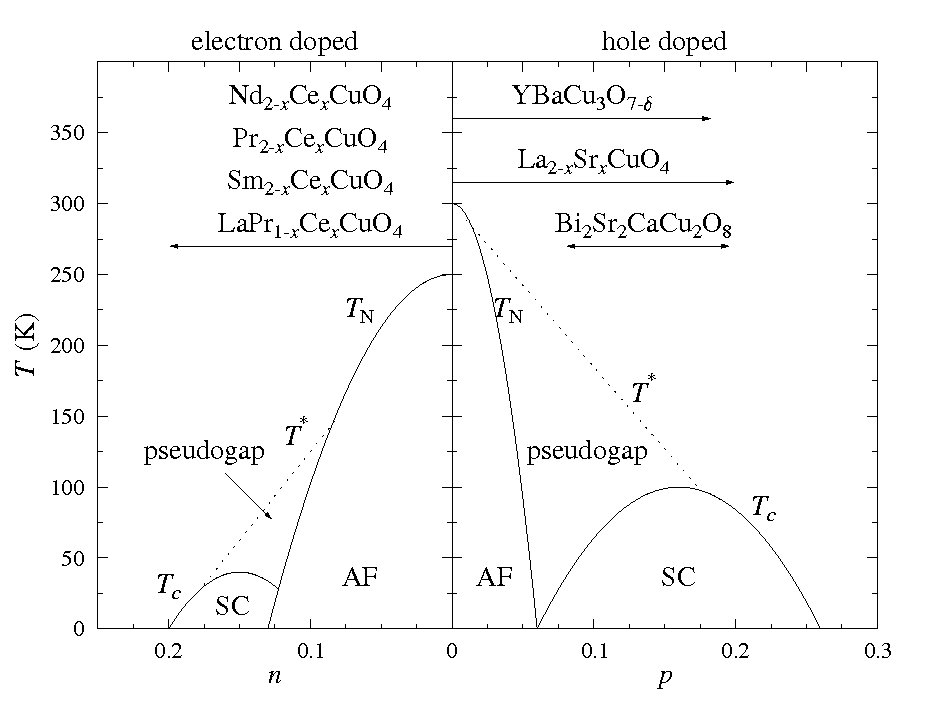
\includegraphics[width=1.0\textwidth]{images/CuPhaseDiag.png}
  \caption{This figure shows a simplified version of the cuprate superconductor phase diagram. \protect\cite{CuPhaseDiag}}
  \label{fig:CuPhaseDiag}
\end{figure}

% Isotopic effects suggested the irrelevance of the lattice, but they are becoming more prominent now.


% First it seemed that in High-Tc the lattice was not that important (isotopic effects at optimal doping).
% Electronic models haven't been completely successful.
In contrast to the BCS theory \cite{Bardeen1957}, the pairing mechanism in the \textit{unconventional superconductors} (cuprates, iron-based and heavy fermion \cite{Pfleiderer2009}) is unknown.
Two leading theories: resonating-valence-bond \cite{?} and spin fluctuation \cite{Scalapino2012} rely heavily on magnetic interactions while mostly ignoring the lattice effects.

% Several experimental observations (lattice and electronic inhomogeneities, phonon spectra and isotopic effects) suggest that lattice plays a fundamental role, altough in a somewhat different fashion than BCS. It seems that below T* there are polaron formation forming the basis state from which superconductivity arises. 

The clues provided by these broken symmetries should yield an understanding of the ground state in this pseudogap phase, its elementary excitations and the appearance of superconductivity at temperatures below the onset of the pseudogap. 

% Electron-lattice correlations could be essential. Maybe in the form of polarons.
% Such correlations can't be adressed with the usual (anti-)adiabatic approximations, so an exact treatment is necessary.
% Exact treatments are computationally expensive so we need to narrow our scope.
% There is evidence of polaronic behaviour in YBCO's O(4)-Cu(1)-O(4).
% A Peierls-Hubbard model has been used there to explain the lattice distortion in terms of bipolarons.
% We explore many other excitations in that model trying to reconcile its predictions with the experimental observations.
% Particular emphasis is given to the isotopic effects because there is controversy around them and they probe the electron-lattice relationship.
% We suggest a possible two-component superconductivity model involving bosonic bi-polaronic objects and free fermions. 
% Chapter outline.


ARPES review: \cite{Damascelli2003}

Pseudogap review: \cite{Timusk1999}

\textit{Inherent inhomogeneity} in HTSC observed by many techniques (see paragraph 2 of \cite{Bussmann-Holder2005}).

The remainder of this introductory chapter is devoted to reviewing some of the experimental results pointing to the importance of considering the lattice and electronic inhomogeneities in the description of superconductivity. 
We start, in section \ref{sec:dynamic_dist} with an overview of the dynamic local lattice distortions in cuprates incluiding the important feature of stripes. 
Afterwards, in section \ref{sec:electronic_inhomogeneity}, we turn our attention to electronic inhomogeneities. 
In sections \ref{sec:phonon_spectra} and \ref{sec:specific_heat} we present some experimental anomalies in the phonon spectra and specific heat respectively and speculate about their possible origin in the mentioned inhomogeneities. 
Next we duscuss some of the controversial experimental results in isotopic effects and ultrafast spectroscopy in sections \ref{sec:isotopic_effects} and \ref{sec:ultrafast_spect} respectively.

In the last part of this introduction we limit the scope of this thesis and present our motivation and approach at describing these dynamic effects (sec. \ref{sec:scope}) and provide an outline of the next chapters (sec. \ref{sec:outline})

\section{Dynamic local lattice distortions}
\label{sec:dynamic_dist}

From https://research-engine.appspot.com/37001/writings/6264610306916352

\begin{quote}
Early determinations of the crystal structure of cuprates by diffraction methods did not show significant distortions associated with either in-plane oxygen atoms or apical oxygen atoms \cite{Capponi1987,Schafer1988}. 
Moreover, the determination of  average bond lengths in diffraction has a precision of $\sim 0.001$\AA \cite{Miceli1988}, significantly higher than the precision in bond length determination that local probes, like extended x-ray absorption fine structure spectroscopy (EXAFS) \cite{Rehr2000}. 
For this reason, early reports of local lattice distortions related to the oxygen atoms  were controversial (see for example \cite{battlog1992lattice,Kwei1990}).

One of the first observations of a local lattice distortion in cuprates was the report of a two-site distribution for the Cu(1)-apical oxygen in YBa$_{2}$Cu$_{3}$O$_{7}$  appearing at temperatures above the superconducting transition temperature, T$_{c}$, using Cu K-edge EXAFS \cite{MustredeLeon1990,Conradson1990}.
This distribution showed two sites separated by $\sim 0.10-0.13$ \AA \cite{Conradson1990,MustredeLeon1992a} that changed into a single site distribution in the vicinity of the superconducting transition temperature. 
These measurements were carried out using polarized x-rays on magnetically oriented powders, an improvement in the technique which allowed to isolate the Cu(1)-axial oxygen [O(4)] (see Fig. 1) signal with an increased sensitivity not achievable for the Cu-O EXAFS signal in other cuprates (see below). 
This result was received with skepticism, based on earlier diffraction results \cite{battlog1992lattice,Kwei1990,Sharma1991} and optical spectroscopy \cite{Thomsen1993}. 
However, it was later confirmed by EXAFS measurements in other oriented samples \cite{Stern1993} and single crystals \cite{Booth1996}, and also found in YBa$_{2}$Cu$_{3}$O$_{6.7}$, YBa$_{2}$Cu$_{3}$O$_{6.5}$ and Co doped YBa$_{2}$Cu$_{3}$O$_{7}$ \cite{MustredeLeon1991}. 
The explanation of the discrepancies between these results with diffraction and optical spectroscopical results lead to the interpretation of  this Cu(1)-O(4) distribution as a dynamical distortion of polaronic origin \cite{MustredeLeon1992}, as discussed in the next section.

Similar two site distributions obtained from EXAFS spectra were found for the Cu(2)-O(4) distribution in Bi$_{2}$Sr$_{2}$CaCu$_{2}$O$_{8}$ \cite{bianconni1992lattice} and in TlBa$_{2}$Ca$_{3}$Cu$_{4}$O$_{11}$ \cite{Allen1991} starting at temperatures above T$_{c}$. 
We note that in these compounds (and other cuprates) the average Cu(2)-O(4) bond length lies between 2.49 and $2.73$ \AA, which is much longer than the Cu(1)-O(4) bond length in YBa$_{2}$Cu$_{3}$O$_{7}$ $(\sim 1.87$ \AA). 
This fact makes more difficult the identification of details of the O(4) distribution due to the stronger mixing of the Cu(2)-O(4) EXAFS signal with those of other atoms and the increased zero point motion of the O(4) atom due to weaker Cu(2)-O(4) bond compared with the Cu(1)-O(4) bond.
For this reason in most EXAFS studies addressing the O(4) motion a gaussian single site broadened distribution has been used, reporting only changes in the width of the distribution as a function of temperature \cite{Booth1995,Oyanagi2007,Zhang2009}.

In plane  Cu(2)-O local lattice distortions were identified in La$_{1.85}$Sr$_{0.15}$CuO$_{4}$ appearing below 100 K \cite{Bianconi1996,Oyanagi2007},  in TIBa$_{2}$CuO$_{6}$ below 120 K \cite{Conradson1997} and in La$_{2}$CuO$_{4.1}$ below 150 K \cite{Lanzara1997,MustredeLeon:xj5003}. 
In this case the observation of such distortions in YBa$_{2}$Cu$_{3}$O$_{7}$ and related compounds becomes more difficult due the similarity  in Cu-O bond lengths in the Cu planes and Cu chains, whose contributions are mixed in the EXAFS signal \cite{Conradson1997,MustredeLeon1992a}.

Until now only in La$_{1.85}$Sr$_{0.15}$CuO$_{4}$ has been possible to identify local lattice distortions involving both in plane oxygen and apical oxygen atoms  \cite{Bianconi1996}. 
We also stress that from all these EXAFS experiments it is only possible to probe with enough detail the nearest neighbor environment around the Cu atoms, thus the spatial extension of the distortions cannot be determined solely from these measurements. 
Additional structural information \cite{Bianconi1996a} is needed to formulate models about the extension of the distortions as discussed in Ref. \cite{Bianconi1996}.

Pair distribution function (PDF) analysis of diffraction, x-ray and neutron inelastic scattering can additionally provide information about the intermediate range (up to $10-15$ \AA)  atomic structure, complementary to the information obtained from EXAFS \cite{Egami2003}. 
PDF results in La$_{1-x}$Sr$_{x}$CuO$_{4}$ \cite{Bozin1999,Bozin2000} indicate that the atomic structure in this material is a combination of nanoscale regions with different local Cu-O environments, in agreement with the model proposed in Ref. \cite{Bianconi1996}. 
A homogeneous structure only appears when dopant concentrations are above $x = 0.25$. 
In this region the electronic behavior can be described in terms of free fermion quasiparticles.

To conclude this survey of local lattice distortion is important to note that the time scale of the EXAFS is such that dynamical distortions can be detected, which depending on the size of the distortion cannot be detected using elastic techniques like neutron diffraction (see section of Results). 
This can explain some of the differences between diffraction and EXAFS results. 
Indeed it has been shown that the two-site O(4) distribution in in Tl$_{2}$Ba$_{2}$CaCu$_{2}$O$_{8}$ could be only detected in a pair distribution function obtained from neutron inelastic scattering but not with that obtained from neutron diffraction \cite{Egami1991}. 
Consequently, it is important to take into account both the spatial resolution and time resolution of the techniques used to study the actual atomic structure of these materials \cite{Mihailovic2005}. 
In the next section we present a microscopic local model that can generate  dynamical local lattice distortions as those observed in these materials, and explain the isotopic effects observed in the pseudogap phase.
\end{quote}

\begin{figure}[ht!]
  \centering
  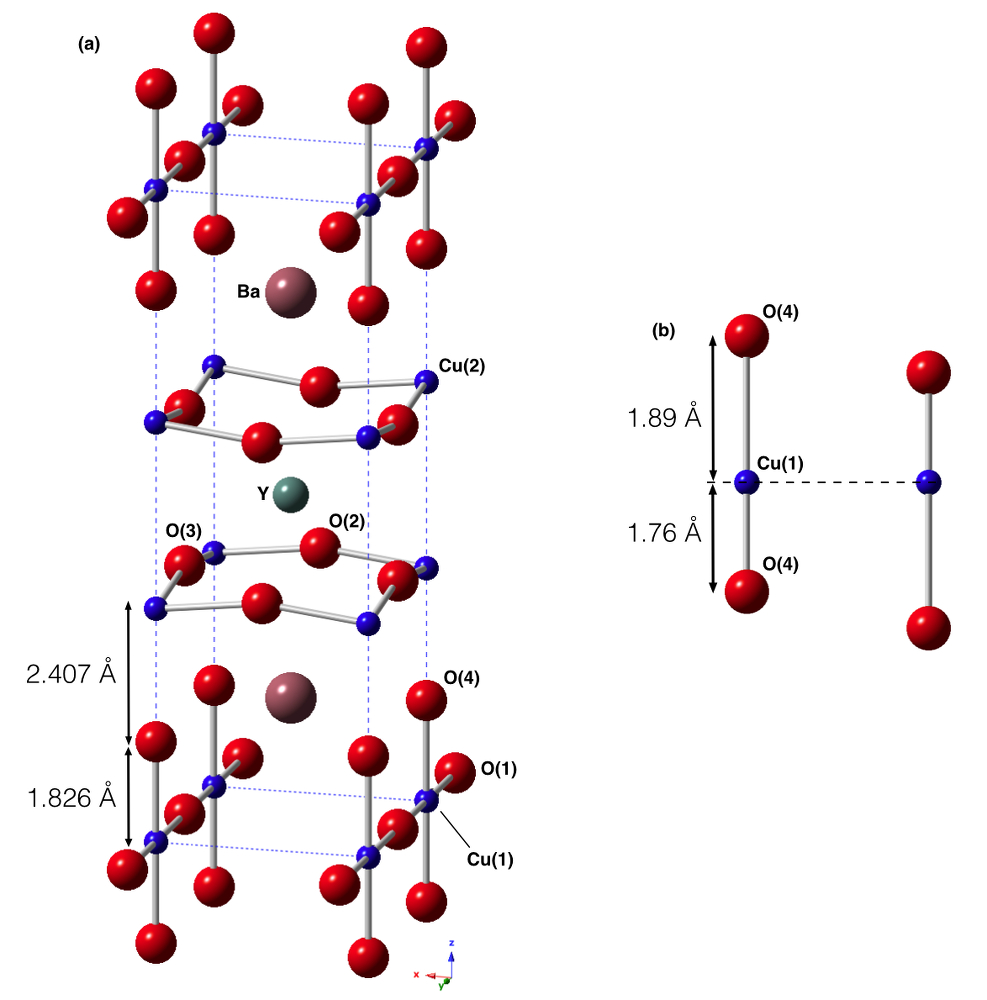
\includegraphics[width=0.8\textwidth]{images/YBCO_O-Cu-O.jpg}
  \caption{\textbf{(a)} Crystal structure of YBa$_{2}$Cu$_{3}$O$_{7}$. The dashed line denotes de unit cell. \textbf{(b)} The two possible configurations in the O(4)-Cu(1)-O(4) cluster due to the split O-Cu bond distances (not to scale).}
\label{fig:YBCO_structure}
\end{figure}

From \cite{Bahrs2004}

\begin{quote}
Samples quenched from high to about room temperature show spontaneous reordering of oxygen atoms in the chain sites on a time scale between hours and days. 
The structural development has been monitored with x-ray and neutron scattering, both verifying a shortening of the crystallographic axes and the formation of superstructure patterns with full and empty chains for values of oxygen deficiency around $\delta \sim  0.5$. 
[...] the critical temperature of the samples was observed to increase, pointing to the close connection between chain length and carrier concentration in the superconducting planes. 
Calculations of the Cu1 valence in different oxygen surroundings explain the charge transfer involved. 
This correlation between structure and electrical properties has also been shown by application of pressure, after which the critical temperature also remains enhanced as long as the sample is kept cool, but relaxes when it is warmed up to room temperature. 
Other metastable effects are induced by illumination, such as persistent photoconductivity, where after exposure to visible light conductivity and, in superconducting samples, critical temperature show a metastable increase.
\end{quote}

\subsection{Stripes}

Review: \cite{Kivelson2003}

\section{Electronic inhomogeneity}
\label{sec:electronic_inhomogeneity}

See introduction of this article: \cite{Ivanov1995}

The parent compounds of cuprate superconductors form ordered crystalline structures and exhibit antiferromagnetic order at low temperatures. 
However,  in compounds like La$_{1.85}$Sr$_{0.15}$CuO$_{4}$ and La$_{2}$CuO$_{4.1}$, the dopant atoms necessary to achieve a superconducting compound are not placed at the crystal symmetry allowed sites yielding to intrinsically structurally inhomogeneous systems\cite{Poccia2011}. 
While in other cases, like YBCO$_{6+\delta}$, extra dopant atoms reside in crystal symmetric positions but the departure from stoichiometry yields compositional disorder\cite{Chen1988} \cite{Andersen1990} with the same consequence. 
In these systems the crystalline translational symmetry is broken. 
Although from the structural inhomogeneity does not necessarily follow an inhomogeneous electronic ground state, for some regions of the phase diagram, depending on the dopant concentration, such state is realized. 
This region of phase space has been identified as the pseudogap phase\cite{Kresin2009} \cite{Muller2007} \cite{Timusk1999}. 
An important consideration is that, although the dopant atoms are at fixed positions, the structural inhomogeneity has a dynamical character\cite{Mihailovic2005} \cite{Bianconi1996} and is present even in compounds with perfect crystallographic symmetry like HoBa$_{2}$Cu$_{4}$O$_{8}$\cite{RubioTemprano2000}. 
In addition to the breaking of the crystalline translational symmetry the pseudogap phase exhibits other broken symmetries. 
Time-reversal symmetry breaking was found using angular resolved photoemission spectroscopy with circularly polarized photons in Bi$_{2}$Sr$_{2}$CaCu$_{2}$O$_{8+\delta}$\cite{Kaminski2002}. 
It was also found, by x-ray absorption spectroscopy, that the crystalline rotational symmetry is broken locally in La$_{1.85}$Sr$_{0.15}$CuO$_{4}$ with alternating regions of tetragonal and orthorhombic symmetry \cite{Bianconi1996}. 
A perspective of the observation of broken symmetries in high-T$_{c}$ superconductors, emphasizing that some of these broken symmetries are hidden from common observational techniques, is discussed in ref.\cite{Chakravarty2011}. The clues provided by these broken symmetries should yield an understanding of the ground state in this pseudogap phase, its elementary excitations and the appearance of superconductivity at temperatures below the onset of the pseudogap. 


\section{Phonon spectra}
\label{sec:phonon_spectra}

Forbidden ir modes only present below T*

\section{Electric resistivity}
\label{sec:resistivity}

T vs T$^2$. See v.g. \cite{Timusk1999}

For a Fermi liquid the dc resistance varies as T$^2$.

\cite{Muller2007}: \textit{At optimum doping, i.e- T$_c$ maximum, and in the normal state, the resistivity increases linearly with temperature}

\section{Specific heat}
\label{sec:specific_heat}

Specific heat: \cite{Loram1993}

For a Fermi liquid the specific heat rises linearly with the temperature.

\section{Isotopic effects}
\label{sec:isotopic_effects}

It is possible to make a site-selective substitution $^{16}$O $\rightarrow$ $^{18}$O in YBCO \cite{Conder1993} allowing a precise study of the isotopic effects. 
This has effects in both the phonon frequencies \cite{Ruani1994} and T$_{c}$ \cite{Zech1994,Cardona1988}. 
The \textit{harmonic} approximation accounts well for the O(2)/O(3) vibrations but it fails for O(4) (see again \cite{Ruani1994})

Noticeable isotopic shifts have been used to identify particular excitations as \textit{phononic} in origin (v.g. \cite{Thomsen1990}) however, we will argue, the converse is not true. 
That is, there can be \textit{phononic} excitations without a measurable isotopic shift.

\section{Ultrafast spectroscopy}
\label{sec:ultrafast_spect}

V.g. \cite{Basov2005} \cite{Smallwood2012} ( http://www.photonics.com/Article.aspx?AID=51474 )

\section{Scope of this thesis}
\label{sec:scope}

% Lattice inhomogeneities limit the applicability of $k$-space formalism.
% Correlated electron-lattice motion prevents the use of Born-Openheimer approximation

Quantum solid-state theory usually assumes a periodic potential however, since these materials are intrinsically inhomogeneous, it is possible that a successful model needs to abandon such assumption. 
This calls into question the applicability of models based on the \textit{reciprocal space} formalism.
Furthermore, some of the experimental results reviewed in the previous secions suggest that the polaronic behaviour must be taken into account.
This correlated electron-lattice movement prevents the use of the Born-Oppenheimer approximation, which splits the system's wavefunction in electronic and lattice factors $\Psi = \psi_{electronic}\psi_{lattice}$.
Some systems with an important electron-lattice interaction can be treated with perturbation theory either assuming a small (adiabatic) or strong (anti-adiabatic) interaction \cite{?}. 
However, it seems that the electron-lattice interaction in the CuO planes for cuprate superconductors falls in the middle of such extremes \cite{MustredeLeon1992} preventing the use of any such approximation.

We are prompted, therefore, to use an exact model free from the approximations described above. 
The computational complexity of exact models forces us to restrict the system under study to a small subset of the whole compound.
In this work we return to a model describing the peculiar polaronic behaviour of the O(4)-Cu(1)-O(4) cluster in YBa$_{2}$Cu$_{3}$O$_{7}$ approximating the cluster as a system with three sites and two holes \cite{MustredeLeon1992}.
Such approximation is justified as the Cu(1)-O(4) bond length (1.83 \AA) is far shorter than the Cu(2)-O(4) bond length ($\sim$ 2.41 \AA) (see Fig. \ref{fig:YBCO_structure}), making charge transfer outside the cluster a much slower process than the charge dynamics inside the cluster. 
This model provides a very simple framework to explore the charge dynamics influenced by the lattice vibrations and has successfully described the split O(4)-Cu(1)-O(4) distance observed by EXAFS experiments (see section \ref{sec:dynamic_dist} above).
Although we cannot directly identify the three site cluster proposed in this model with a particular structure of the CuO plane, the general approach of charge transfer between hole rich regions and hole poor regions in the plane coupled to the lattice degrees of freedom is still valid, hence the general conclusions we draw from this model applicable to describe the structure of the CuO plane.

It has been found that superconductivity occurs in the Cu(2)-O(2,3) planes rather than the Cu(1)-O(1,4) chains partially addressed by the model under study in this work.
This raises a question about the relevance of the polaronic behaviour, es explored with this model, to superconductivity.
It is indeed beyond the capability of such a simple model to address the nature of high-temperature superconductiity.
However, it is possible that the polaronic objects in the Cu(1)-O(1,4) chains are capable of providing a pairing mechanism for the Cooper pairs in the Cu(2)-O(2,3) planes.
This will point to a \textit{two component superconductivity} theory similar to some current proposals \cite{?}

\section{Thesis outline}
\label{sec:outline}

% I need to rewrite this section once I finish everything else...

In chapter \ref{chap:model} we describe in detail the three sites Peierls-Hubbard model used to describe the O-Cu-O cluster in YBCO with some of its generalities. 
The rich phenomenologies of the ground and excited states of this model are explored in the remaining chapters. 
Chapter \ref{chap:ground} is devoted to the ground state (identified also as the \textit{polaron formation energy}). 
Next, in chapter \ref{chap:results}, we describe the next few infrared-allowed excitations. 
Finally, in chapter \ref{chap:electronic}, we turn our attention to the first \textit{electronic} excitation of this model. 
We conclude this work, in chapter \ref{chap:conclusions}, with some conclusions and perspectives.

\chapter{Peierls-Hubbard model}
\label{chap:model}

As mentioned in section \ref{sec:scope}, treatments based in the adiabatic and antiadiabatic approximations are unable to describe properly the correlated electron-lattice motion in cuprate's Cu-O bonds.
An alternative to overcome this limitation is an exact treatment of a reduced system.
In this thesis we focus on the O(4)-Cu(1)-O(4) cluster in YBa$_2$Cu$_3$O$_7$.
We approximate this local environment as a three site cluster with two holes. 
Such approximation is justified as the Cu(1)-O(4) bond length (1.83 \AA) is far shorter than the Cu(2)-O(4) bond length ($\sim 2.41$ \AA) (see figure \ref{fig:YBCO_structure}), making charge transfer outside the cluster a much slower process than the charge dynamics inside the cluster. 
Although we cannot directly identify the three site cluster proposed in this model with a particular structure of the CuO plane, the general approach of charge transfer between hole rich regions and hole poor regions in the plane coupled to the lattice degrees of freedom is still valid, hence the general conclusions we draw from this model applicable to describe the structure of the CuO plane.

This thesis is based in a thorough analysis of that model hamiltonian so we devote this chapter to a detailed description of its components.
In section \ref{sec:hamiltonian-and-basis} we describe the hamitlonian and the basis used. 
Section \ref{sec:isotopic-model} reviews a method of incorporating isotopic substitutions in this model and defines \textit{isotopic shifts} in this context.
In section \ref{sec:lattice-distortions} we discuss a method of calculating real-space lattice distortions.
Next, in section \ref{sec:electronic-projection}, we describe a projection into definite electronic occupation states.
Section \ref{sec:model-parameters} reviews some literature suggesting possible choices of parameters and lists the parameters used in this work.
We review in section \ref{sec:classification} a method for identifying and classifiying the different excitations in this model.
Finally, section \ref{sec:comp_details} gives some computational details about our calculations.

\section{Hamiltonian and basis set}
\label{sec:hamiltonian-and-basis}

To describe two holes in the O(4)-Cu(1)-O(4) cluster with an electron-lattice (phonon) correlated movement we use a hamiltonian consisting of three parts:

\begin{equation}
  \label{eq:full-hamiltonian}
  H = H_{el} + H_{ph} + H_{el-ph}
\end{equation}

\noindent corresponding to the electronic contribution, the phonon energies and the electron-phonon (lattice) coupling, respectively \cite{Salkola1994}. 
The electron-phonon coupling term deviates this model from the Born-Oppenheimer (adiabatic) approximation and prevents the separation of hamiltionan eigenstates, $\Psi$, as products of purely electronic and phononic parts, $\Psi=\psi_{el}\psi_{ph}$, unless $H_{el-ph}=0$.
Nonetheless, as it will be discussed in section \ref{sec:classification}, even for coupling values greater than zero the hamiltonian eigenstates can be interpreted as mainly \textit{electronic} or \textit{phononic} in nature.

The electronic part is modeled as a single band Hubbard model for three sites with two holes in it. 
We only consider the two holes as having opposite spin because the energies of states with two charges with the same spin are much greater.
Explicitly, $H_{el}$ is written as

\begin{equation}
  \label{eq:electronic-part}
  H_{el} = \sum_{\sigma,i=1}^3 E_i n_{\sigma i} 
        + U\sum_{i=1}^3 n_{i\downarrow}n_{i\uparrow} 
        + t\sum_{\sigma} \left(c_{1\sigma}^\dagger c_{2\sigma} + c_{2\sigma}^\dagger c_{3\sigma} + H.c. \right)
\end{equation}

\noindent where we denoted $n_{i\sigma}=c_{i\sigma}^\dagger c_{i\sigma}$ as the hole-number operator with $c_{i\sigma}^\dagger$ creating a hole with spin $\sigma = \uparrow, \downarrow$ and $c_{i\sigma}$ destroying it; the site index $i=1,2,3$ indicates the two oxygen sites [O(4)] when  $i=1,3$ and the only copper site [Cu(1)] when $i=2$. 
The site energies are parametrized with $E_1=E_3=-E_2 \equiv E_0$.\footnote{In \cite{Salkola1995} the authors consider an example of \textit{disorder} in this system by letting $E_1\neq E_3$.}
$U$ is the on-site Coulomb interaction and $t$ is the hopping energy between two adjacent sites. 

For the lattice  part of the Hamiltonian, $H_{ph}$, we consider both symmetric (Raman) and antisymmetric (infrared) modes described by boson operators $b_R$ and $b_{ir}$ and bare frequencies $\omega_R$ and $\omega_{ir}$ respectively,\footnote{Unlike previous publications, here we include the \textit{zero-point energy} for both phonon modes. 
For most cases this is not needed since the excitation's energies are calculated relative to the ground state but, in chapter \ref{chap:ground} we study the ground state energy itself where this contribution is important}

\begin{equation}
 \label{eq:phonon-part}
 H_{ph} = \hbar \omega_{ir}\left(b_{ir}^\dagger b_{ir}+\frac{1}{2}\right) + \hbar \omega_R \left( b_R^\dagger b_R + \frac{1}{2}\right)
\end{equation}


\begin{figure}[ht!]
  \centering
  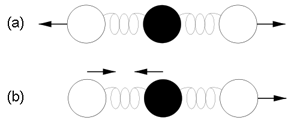
\includegraphics[width=0.5\textwidth]{images/CO2-vibrations.png}
  \caption{Schematic showing the \textbf{(a)} symmetric (Raman) and \textbf{(b)} asymmetric (infrared) vibrational modes for the CuO$_2$ cluster.}
  \label{fig:CO2-vibrations}
\end{figure}

 
The electron-lattice coupling term, $H_{el-ph}$ is introduced through the change in interatomic distances generated by Coulomb repulsion between different sites coupled with the Raman and infrared phonon modes,
 
\begin{equation}
  \label{eq:coupling-part}
  H_{el-ph} = \lambda_{ir}(b_{ir} + b_{ir}^\dagger)(n_3 - n_1) + \lambda_R (b_R + b_R^\dagger)(n_1 + n_3-s_0)
\end{equation}

Here $s_0$ is a constant used to avoid artificial shrinking of the cluster\footnote{This term is written slightly different in some publications, like \cite{MustredeLeon1992}, however both versions can be related noticing that $3 (n_1+n_3-4/3)=n_1-2n_2+n_3$.}. 
For consistency with other works \cite{MustredeLeon1992,DeLeon1999,Leon2008,MirandaMena2007} we fix $s_0=4/3$.

% Describe how the different values for n_1, n_2, n_3 couple to phonons. Maybe include a figure here.

One simple basis set for this system can be denoted by is $\{\ket{e_1,e_2,ir,R}: e_1,e_2=1,2,3; ir,R=1,2,\ldots\}$ with $e_k$ being the position of the $k$-th hole, $ir$ the number of \textit{infrared} phonons and $R$ the number of \textit{Raman} phonons. 
This basis is infinite dimensional however, as discussed in section \ref{sec:comp_details}, for the lower energy excitations the eigenvalues and eigenvectors are well described using a basis with only a few phononic labels.

To build the hamiltonian we need to assign an integer label $l$ to each basis state. 
This can be achieved with the mapping

\begin{equation}
  \label{eq:label}
  l = e_1 + 3(e_2 - 1) + 9\ ir + 9\ R (n_{ir} +1)
\end{equation}

\noindent with $n_{ir}$ being the total number of infrared phonons under consideration.

\section{Isotopic substitutions}
\label{sec:isotopic-model}

The effects of isotopic substitutions in cuprate superconductors have been extensively studied and reveal fundamental properties of the material (see section \ref{sec:isotopic_effects}). 
It is, therefore, of interest to model these effects on the three sites cluster we are studying.
Changing the atomic mass in any of the three sites of the model should change the phonon frequencies $(\omega_{ir},\omega_R$) in (\ref{eq:phonon-part}) and the coupling constants $(\lambda_{ir},\lambda_R)$ in (\ref{eq:coupling-part}).

\subsection{A classical model for the atomic vibrations}

To model the effect of this change in mass we describe the motion of the nuclei as three masses attached by springs (see figure \ref{fig:3-masses-2-springs}) and find the normal vibrational modes using classical mechanics.

\begin{figure}[ht!]
\centering
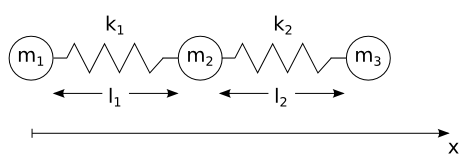
\includegraphics[width=0.6\textwidth]{images/3-masses-2-springs-linear.png}
\caption{Diagram for 3 masses attached with springs representing the nuclei motion.}
\label{fig:3-masses-2-springs}
\end{figure}

Consider 3 masses $m_i,\ i=1,2,3$ attached linearly by two springs of constants $k_1$ and $k_2$ and rest length of $l_1$ and $l_2$ respectively (later we will let $ m_1=m_3$, $ k_1=k_2$ and $l_1=l_2$). 
We will look only at the motion in the longitudinal direction so we attach a reference frame and call $ x_i$ ($i=1,2,3$) the coordinate describing the position of $m_i$.
A lagrangian $L$ for this system is 

\begin{align}
L & = T-V\\
  & = \frac{1}{2}\sum_{i=1}^3 m_i \dot{x}_i^2 - \frac{1}{2}k_1(l_1-(x_2-x_1))^2+\frac{1}{2}k_2(l_2-(x_3-x_2))^2
\end{align}

It will be more convenient to change the $x_i$ coordinates to another set reflecting only the displacements from the equilibrium position.
That is, we define new coordinates $\eta_i$ such that $(x_1,x_2,x_3)=(\eta_1,l_1+\eta_2,l_1+l_2+\eta_3)$. 
In this coordinate system the lagrangian looks simpler

\begin{equation}
  L= \frac{1}{2}\sum_{i=1}^3 m_i \dot{\eta}_i^2-\frac{1}{2}k_1(\eta_1-\eta_2)^2+\frac{1}{2}k_2(\eta_2-\eta_3)^2
\end{equation}

The potential energy is a quadratic function of the $\eta_i$ displacements so we can write it in the general form $V=\frac{1}{2}\sum_{i,j}V_{ij}\eta_i\eta_j$ where $V_{ij}$ are the elements of the matrix defined as

\begin{equation}
  (V_{ij})=\left( \begin{array}{ccc} k_1 & -k_1 & 0 \\ -k_1 & k_1+k_2 & -k_2 \\ 0 & -k_2 & k_2 \end{array} \right)
\end{equation}

The dynamics of the system is determined by the Euler-Lagrange equations,

\begin{align}
  0 & = \frac{d}{dt}\frac{\partial L}{\partial \dot{\eta}_s}-\frac{\partial L}{\partial \eta_s} \label{eq:EulLag1} \\
    & = m_s \ddot{\eta}_s + \sum_i V_{is} \eta_i \label{eq:EulLag2}
\end{align}

\noindent for $s=1,2,3$. 
We can propose an oscillatory solution of the form $\eta_i=a_ie^{i\omega t}$, understanding that only the real part of this equations describe the real motion of the cluster. 
Substituting this solution into the equations of motion (\ref{eq:EulLag2}), after removing the common exponential factor, gives

\begin{equation}
  0=\sum_i V_{is}a_i-\omega^2m_sa_s
\end{equation}

which can be arranged as a matrix

\begin{equation}
  \left( 
    \begin{array}{c} 
      0\\ 0\\ 0 
    \end{array}
  \right) = (V_{ij}) \left(
    \begin{array}{c}
      a_1 \\ a_2 \\ a_3 
    \end{array}
  \right) - \omega^2 \left(
    \begin{array}{ccc}
      m_1 & 0 & 0 \\ 0 & m_2 & 0 \\ 0 & 0 & m_3
    \end{array}\right) \left(
    \begin{array}{c} 
      a_1 \\ a_2 \\ a_3 
    \end{array}
  \right)
\end{equation}

Substituting the actual values for $(V_{ij})$:

\begin{equation}
  \left( 
    \begin{array}{c}
      0\\ 0\\ 0
    \end{array}
  \right) 
  = \left(
    \begin{array}{ccc}
      k_1-\omega^2m_1 & -k_1 & 0 \\ -k_1 & k_1+k_2-\omega^2m_2 & -k_2 \\ 0 & -k_2 & k_2-\omega^2m_3 
    \end{array}
  \right) 
  \left(
    \begin{array}{c}
      a_1 \\ a_2 \\ a_3 
    \end{array}
  \right)
\end{equation}

In order to have a non-trivial solution we require the determinant of that matrix to be zero

\begin{equation}
  \label{eq:det}
  \begin{split}
    0 = & (k_1-\omega^2m_1)(k_1+k_2-\omega^2m_2)(k_2-\omega^2m_3) \\
        & -k_1^2(k_2-\omega^2m_3)-k_2^2(k_1-\omega^2m_1)
  \end{split}
\end{equation}

\noindent which is a third order alebraic equation for $\omega^2$ with 3 solutions for $\omega$.
To simplify the calculation we take now into consideration the details of our problem, that is, we consider $m_1 = m_3 \equiv m_O$, $m_2 \equiv m_{Cu}$ and $k_1 = k_2 \equiv k$. 
With this considerations, (\ref{eq:det}) simplifies to

\begin{align}
  \label{eq:omegas}
  0 & = (k-\omega^2m_O)^2(2k-\omega^2m_{Cu})-2k^2(k-\omega^2m_O) \\
    & = (k-\omega^2m_O)[(k-\omega^2m_O)(2k-\omega^2m_{Cu})-2k^2]
\end{align}

\noindent from which we can observe one solution

\begin{equation}
  \omega^2= \frac{k}{m_O}
\end{equation}

\noindent corresponding to the symmetrical (Raman) vibrational mode, denoted by $\omega_{R}$ in \ref{eq:phonon-part}, since it doesn't depend on $m_{Cu}$.
The other two frequencies are obtained from the remaining factor in \ref{eq:omegas},

\begin{equation}
  \begin{split}
    0 & = (k-\omega^2m_O)(2k-\omega^2m_{Cu})-2k^2 \\
      & = 2k^2-k\omega^2m_{Cu}-2k\omega^2m_O+\omega^4m_Om_{Cu}-2k^2 \\
      & = \omega^2[\omega^2m_Om_{Cu}-k(m_{Cu}+2m_O)]
  \end{split}
\end{equation}

\noindent from here we obtain the uninteresting $\omega^2=0$ and

\begin{equation}
  \omega^2 = \frac{k(m_{Cu}+2m_O)}{m_Om_{Cu}}
\end{equation}

This is the frequency of the asymmetric (infrared) vibrational mode, denoted by $\omega_{ir}$ in (\ref{eq:phonon-part}).
Summarizing this part, we have found the dependency of the phonon frequencies $\omega_{ir}$ and $\omega_R$ with the atomic masses for the oxygen $m_O$ and copper $m_{Cu}$ atoms in the following way

\begin{equation}
  \label{eq:omegaR}
  \omega_{R}= \sqrt{\frac{k}{m_O}}
\end{equation}

\begin{equation}
  \label{eq:omegair}
  \omega_{ir} = \sqrt{\frac{k(m_{Cu}+2m_O)}{m_Om_{Cu}}}
\end{equation}

\noindent for some constant $k$.
Also, from here we identify the reduced masses for each vibrational mode

\begin{equation}
  \label{eq:redMassR}
  m_R \equiv m_O \simeq 16.0\ u \simeq 2.6568 \times 10^{-26} kg
\end{equation}

\begin{equation}
  \label{eq:redMassIr}
  m_{ir} \equiv \frac{m_Om_{Cu}}{m_{Cu}+2m_O} \simeq 10.64\ u \simeq 1.7668 \times 10^{-26}kg
\end{equation}

\subsection{Change in the coupling constants}

Also, the coupling parameters depend on $m_O$\cite{?}:

\begin{equation}
  \label{eq:ir-coupl-isot}
  \lambda_{ir}\propto (m_O\omega_{ir})^{-1/2}
\end{equation}

\begin{equation}
  \label{eq:Ram-coupl-isot}
  \lambda_R\propto (m_O\omega_{R})^{-1/2}
\end{equation}


\subsection{Effects of changing the oxygen mass}

From the discussion in the previous sections, it can be seen that an oxygen isotpe substitution, $^{16}$O $\rightarrow$ $^{18}$O ammounts to a change in the frequencies  $(\omega_{ir}$, $\omega_R)$ and the coupling constants $(\lambda_{ir},\lambda_R)$.
We now turn to the task of finding the ammount of such changes.
Denoting as $\omega^{(16)}$ and $\omega^{(18)}$ the phonon frequencies for a cluster with $^{16}$O and $^{18}$O respectively, from (\ref{eq:omegair}, \ref{eq:omegaR}) we can calculate the ratios

\begin{align}
  \omega^{(16)}_{ir}/\omega^{(18)}_{ir}
  & =\sqrt{\left(\frac{m_{^{18}O}}{m_{^{16}O}}\right)\left(\frac{m_{Cu}+2m_{^{16}O}}{m_{Cu}+2m_{^{18}O}}\right)} \\
  \omega^{(16)}_{R}/\omega^{(18)}_{R}
  & =\sqrt{\frac{m_{^{18}O}}{m_{^{16}O}}}
\end{align}

Taking the actual values for copper and oxygen, $m_{Cu}=63.546u$, $m_{^{16}O}=15.995u$ and $m_{^{18}O}=17.999u$, we obtain

\begin{equation}
  \label{eq:omega-ir-isot}
  \omega^{(16)}_{ir} / \omega^{(18)}_{ir} \simeq 1.039
\end{equation}

\begin{equation}
  \label{eq:omega-R-isot}
  \omega^{(16)}_{R} / \omega^{(18)}_{R} \simeq 1.061
\end{equation}

Similarly, for the coupling constants $\lambda_{ir}$ and $\lambda_R$, from (\ref{eq:ir-coupl-isot}, \ref{eq:Ram-coupl-isot}) we can observe that

\begin{equation}
  \label{eq:lambda-ir-isot}
  \lambda_{ir}^{(16)}/\lambda_{ir}^{(18)}=\sqrt{\frac{m_{^{18}O}\omega_{ir}^{(18)}}{m_{^{16}O}\omega_{ir}^{(16)}}}\simeq 1.0407
\end{equation}

\noindent and similarly for the Raman coupling constant

\begin{equation}
  \label{eq:lambda-Ram-isot}
  \lambda_R^{(16)} / \lambda_R^{(18)} \sqrt{\frac{m_{^{18}O}\omega_{R}^{(18)}}{m_{^{16}O}\omega_{R}^{(16)}}} \simeq 1.0299
\end{equation}

Summarizing, to model an isotopic substitution $^{16}$O$\rightarrow ^{18}$O we need to adjust the vibrational frequencies and coupling constants according to equations (\ref{eq:omega-ir-isot}-\ref{eq:lambda-Ram-isot})

\subsection{Definition of isotopic shifts}

% Motivation missing

We define the relative isotopic shift for an excited state $i$ as 

\begin{equation}
  \label{eq:isot-shift-def-exc}
  \Delta_i = \frac{\omega_i(^{16}O)- \omega_i(^{18}O)}{\omega_i(^{16}O)} \times 100
\end{equation}

\noindent where the energies $\omega_i$ are referred to the corresponding ground state.

For the ground state we define the energy isotopic shift $\Delta_g$ in a similar way but with the energies measured relative to the uncoupled system, that is, the system with $\lambda_{ir}=\lambda_R=0$,

\begin{equation}
  \label{eq:isot-shift-def-grd}
  \Delta_g = \frac{\Delta\omega_g(^{16}O)- \Delta\omega_g(^{18}O)}{\Delta \omega_g(^{16}O)} \times 100
\end{equation}

\noindent where $\Delta\omega_g \equiv \omega_g - \omega_g(\lambda_{ir}=0, \lambda_R=0)$. 
For the calculation of $\Delta_g$ it is essential to include the \textit{zero point energy} in the phononic part (\ref{eq:phonon-part}) which is usually not taken into account.

\section{Lattice distortions}
\label{sec:lattice-distortions}

To understand the lattice distortion for excitations in the model hamiltonian (\ref{eq:full-hamiltonian}) it is useful to find the projection of a given state to real space atomic coordinates. 
In a simple quantum harmonic oscillator with mass $m$ and frequency $\omega$ the creation and annihilation operators, $a^\dagger$ and $a$, are related to the real-space coordinate $x$ as

\begin{equation}
  \label{eq:harmOscRel}
  x=\sqrt{\frac{\hbar}{2m\omega}}\left(a+a^\dagger\right)
\end{equation}

If we assume that phonon modes in our model hamiltonian (\ref{eq:phonon-part}) behave as quantum harmonic oscillators, we can define symmilar real space operators ($u_r,u_{ir}$) in terms of the bosonic creation and annihilation operatos ($b^\dagger,b$) for both, infrared and Raman, vibrational modes. 
These operators, called \textit{phonon coordinates}, are also related to the positions $x_i$ of the three sites in the cluster \cite{MustredeLeon1992},

\begin{equation}
  \label{eq:uR}
  u_R \equiv \left(\frac{\hbar}{2 m_R \omega_R}\right)^{1/2}(b_R^\dagger + b_R) = \frac{x_3 - x_1}{\sqrt{2}}
\end{equation}

\begin{equation}
  \label{eq:uir}
  u_{ir} \equiv \left(\frac{\hbar}{2 m_{ir} \omega_{ir}}\right)^{1/2}(b^\dagger_{ir}+b_{ir}) = \frac{ x_1 + x_3 - ( 2 m_O/m_{Cu})x_2}{(2 + 4 m_O/m_{Cu})^{1/2}}
\end{equation}

The reduced masses $m_R$ and $m_{ir}$ are determined in equations (\ref{eq:redMassR}, \ref{eq:redMassIr}).
In a quantum harmonic oscillator an energy eigenfunction, $\ket{n}$, has a projection into the real space coordinate $x$ given in terms of a Hermite polynomial $H_n(x)$ of degree $n$ in the following way,

\begin{equation}
  \label{eq:harmOscProj}
  \braket{x}{n} 
  \equiv \psi_n(x) 
  = \frac{1}{\sqrt{2^n n!}} \left(\frac{m \omega}{\pi \hbar}\right)^{1/4}
  \exp\left(-\frac{m \omega x^2}{2 \hbar}\right) H_n\left( \sqrt{\frac{m \omega}{\hbar}} x \right) 
\end{equation}


For an arbitrary wavefunction $\ket{\psi} = \sum_n \braket{n}{\psi} \ket{n}$ the projection in real space is $\braket{x}{\psi} = \sum_n \braket{n}{\psi} \braket{x}{n}$ with $\braket{x}{n}$ given by \ref{eq:harmOscProj}.

For the model hamiltonian (\ref{eq:full-hamiltonian}), as discussed in section \ref{sec:hamiltonian-and-basis}, a possible basis set is given by the functions ${| e_1, e_2, ir, R \rangle}$ with $e_i$ the position of the $i$-th electron and $ir$, $R$ the number of infrared and Raman phonons respectively. 
Thus an arbitrary wavefunction in this system, $\ket{\psi}$, can be expanded as

\begin{equation}
  \label{eq:wf-phonon-base}
  \ket{\psi}=\sum_{e_1,e_2,ir,R} \braket{e_1,e_2,ir,R}{\psi}\ket{e_1,e_2,ir,R}
\end{equation}

\noindent and we can make the partial projection into the phonon coordinates $(u_{ir},u_R)$ as defined by (\ref{eq:uR},\ref{eq:uir})

\begin{equation}
  \label{eq:wf-expansion}
  \braket{u_{ir},u_R}{\psi}=\sum_{e_1,e_2,ir,R} \braket{e_1,e_2,ir,R}{\psi}\braket{u_{ir},u_R}{ir,R}\ket{e_1,e_2}
\end{equation}

\noindent where we have denoted $\braket{u_{ir},u_r}{e_1,e_2,ir,R}=\braket{u_{ir},u_R}{ir,R}\ket{e_1,e_2}$. 
The term $\braket{u_{ir},u_r}{ir,R}$ is similar to (\ref{eq:harmOscProj}) but considering both phonon modes:

\begin{equation}
  \label{eq:hermite-expansion}
  \braket{u_{ir},u_r}{ir,R}  = \frac{\left(m_{ir}m_R\right)^{1/4}}{\sqrt{2^{(ir+R)} ir!R!\pi\hbar}}
  \exp\left(-\frac{\tilde{u}_{ir}^2 + \tilde{u}_R^2}{2}\right) 
  H_{ir}\left(\tilde{u}_{ir} \right)H_{R}\left(\tilde{u}_{R} \right)
\end{equation}

\noindent where we have defined the normalized coordinates,

\begin{equation}
  \label{eq:uTildeDef}
  \tilde{u}_j \equiv \sqrt{\frac{m_j\omega_x}{\hbar}}\ u_j
\end{equation}

\noindent for $j=ir,R$. 
Now, from (\ref{eq:wf-expansion}), the probability amplitude of findind a state $\ket{\psi}$ proyected into phonon coordinates $(u_{ir},u_R)$ for a given site occupation $(e_1,e_2)$ is

\begin{equation}
  \begin{split}
    & \left|\braket{e_1,e_2,u_{ir},u_R}{\psi}\right|^2 \\
    & \ \ = \left|\sum_{e_1',e_2',ir,R}\braket{e_1,e_2,ir,R}{\psi}\braket{u_{ir},u_R}{ir,R}\braket{e_1,e_2}{e_1',e_2'}\right|^2 \\
    & \ \ = \left|\sum_{ir,R}\braket{e_1,e_2,ir,R}{\psi}\braket{u_{ir},u_R}{ir,R}\right|^2
  \end{split}
\end{equation}

Finally, the probability amplitude of finding a system in the state $\ket\psi$ with phonon coordinates ($u_{ir},u_R$) irrespective of the electronic configuration is given by the sum over the electronic degrees of freedom on the previous equation,

\begin{equation}
  \label{eq:phonon-coord-projection}
  \begin{split}
    \left|\psi(u_{ir}, u_R)\right|^2 & \equiv \sum_{e_1,e_2}\left|\braket{e_1,e_2,u_{ir},u_R}{\psi}\right|^2 \\
    & = \sum_{e_1,e_2} \left|\sum_{ir,R}\braket{e_1,e_2,ir,R}{\psi}\braket{u_{ir},u_R}{ir,R}\right|^2
  \end{split}
\end{equation}

\noindent with $\braket{u_{ir},u_R}{ir,R}$ given by (\ref{eq:hermite-expansion}).

The projection \ref{eq:phonon-coord-projection} allows us to calculate the probability amplitude of finding a specific distortion in the atomic coordinates for the O-Cu-O cluster.
With the atomic coordinates $x_i$, as defined in section \ref{sec:isotopic-model}, the difference $d$ in between one O-Cu bond and the other is

\begin{equation}
  \label{eq:bondDiff}
  d =  (x_3 - x_2) - (x_2 - x_1) = x_1 + x_3 - 2x_2 
\end{equation}

The $x_i$ coordinates are varying at all times but taking an instant in which $x_2=0$ we can simplify (\ref{eq:bondDiff}) to

\begin{equation}
  \label{eq:bondDiffSimpl}
  d = x_1+x_3
\end{equation}

From $u_{ir}$'s definition in (\ref{eq:uir}),

\begin{equation}
  \label{eq:uirSimpl}
  u_{ir}=\frac{x_1+x_3}{\left( 2+4 m_O/m_{Cu} \right)^{1/2}}
\end{equation}

Now, using (\ref{eq:bondDiffSimpl}) and (\ref{eq:uirSimpl}), we find that

\begin{equation}
  \label{eq:uirvsd}
  u_{ir} = \frac{d}{\left( 2+4 m_O/m_{Cu} \right)^{1/2}}
\end{equation}

\noindent or, solving for $d$,

\begin{equation}
  \label{eq:dvsuir}
  d=\sqrt{2}\left(1 + 2\frac{m_O}{m_{Cu}} \right)^{1/2}u_{ir}
\end{equation}

\noindent which is a relationship between the phonon coordinates, that can be calculated from the model's eigenfunctions, and the observable lattice distortion. 
Equation (\ref{eq:dvsuir}) allows a conection between this model hamiltonian and a specific experimental observation. 
It is this relationship that helps fixing the free coupling parameters $\lambda_{ir}$ and $\lambda_R$ in this model.

\section{Projection into states with definite electron occupation numbers}
\label{sec:electronic-projection}

Eigenstates of the hamltonian \ref{eq:full-hamiltonian}, in general, have delocalized charges.
To understand charge dynamics according for each excitation it is useful to project the eigenstates into the definite electron occupation basis states discussed in section \ref{sec:hamiltonian-and-basis}.
The basis set we are using ($\{\ket{e_1,e_2,ir,R}\}$) has sharp values for the hole number operator on each site for a given number of infrared $ir$ and Raman $R$ phonons. 
Thus, to find the probability $P(e_1,e_2)$ of finding one hole in site $e_1$ and the other on site $e_2$, we need only to sum over the infrared and Raman phonons of the system,

\begin{equation}
  \label{eq:electron-occupation}
  P(e_1,e_2)=\sum_{ir,R} \left| \braket{e_1,e_2,ir,R}{\psi} \right|^2
\end{equation}

From the labeling convention stated in (\ref{eq:label}) we can visualize the nine possible combinations of hole occupancy. 
Denoting, for example, $e_1$ as $\uparrow$ and $e_2$ as $\downarrow$ we have the following combinations:

\begin{equation}\label{eq:basis-set}
\begin{array}{cccc}
1= & \uparrow \downarrow & - & - \\
2= & \uparrow & \downarrow & - \\
3= & \uparrow & - & \downarrow \\
4= & \downarrow & \uparrow & - \\
5= & - & \uparrow \downarrow & - \\
6= & - & \uparrow & \downarrow \\
7= & \downarrow & - & \uparrow \\
8= & - & \downarrow & \uparrow \\
9= & - & - & \uparrow \downarrow 
\end{array}
\end{equation}

Since the model hamiltonian (\ref{eq:full-hamiltonian}) does not distinguish spin and the cluster is symmetrical, states (1, 9) are equivalent, as well as (2, 4, 6, 8) and (3, 7).

\section{Choice of parameters}
\label{sec:model-parameters}

To choose values for this model we take representative values guided from local-density approximations \cite{Pickett1989}. 
In particular Ref. \cite{DeWeert1989}, using a tight-binding model, reports a band energy of $E_0$ = 0.35 eV and a hopping parameter of $t=0.43-0.74$ eV, for Cu(1)-O(4) sites.
The on-site Coulomb repulsion in La$_2$CuO$_4$, $U$  is estimated to be in the range $4.0-10.5$ eV, \cite{Hybertsen1989}. 

The bare phonon frequencies are fixed to values found experimentally in optical and inelastic neutron scattering experiments $\omega_R = 500$ cm$^{-1}$ and $\omega_{ir} = 612.4$ cm$^{-1}$ for YBa$_2$Cu$_3$O$_7$ \cite{?}.

In order to consider the simplest possible model we make the further assumption of taking the on-site Coulomb repulsion in the copper and oxygen sites to be equal with no nearest neighbor Coulomb repulsion. 
We also use a single hopping parameter $t$ and ignore hopping between the two oxygen sites. 
Since only the coupling between the asymmetric mode and the charge motion leads to a measurable lattice distortion, with two Cu–O bond lengths, we only consider the effect of the variation in the electron–lattice coupling constant with the antisymmetric mode, $\lambda_{ir}$, and we set the electron-lattice coupling with the symmetric mode, $\lambda_R$ , as zero \cite{Salkola1995}. 
The inclusion of those considerations in the model, or other choices of parameters (e.g. \cite{Salkola1994, Salkola1995}) yield very similar results.
The relevant value for the coupling $\lambda_{ir}$ is determined using equation \ref{eq:dvsuir}; it is chosen such that the ground state has a maximum probability density at a $u_{ir}$ that reproduces the observed lattice distortion of 0.13 \AA \cite{?}.
In this work we use the same parameters as \cite{DeLeon1999, Leon2008, MirandaMena2007,Mena2006}, namely:

\begin{itemize*}
\item On-site Coulomb repulsion for O(4) and Cu(1) sites: $U=7$ eV
\item Nearest-neighbor hopping: $t=0.5$ eV
\item Band energy for O(4) and Cu(1) sites: $E_0=0.5$ eV
\item Bare phonon frequency for the Raman mode: $\omega_R=500$ cm$^{-1}$
\item Bare phonon frequency for the infrared mode: $\omega_{ir}=612.4$ cm$^{-1}$
\end{itemize*}

As previously stated, some variation in the parameter space has been explored without changes in the basic phenomenology. Table \ref{tab:parameters} shows the parameters for this model used in other publications\footnote{It seems that the reported values for the phonon frequencies in \cite{Salkola1994, Salkola1995} are erroneous since they show $\omega_R > \omega_{ir}$ and they are inconsistent from what can be observed in Fig. 1 of \cite{Salkola1994} at $\lambda_{ir}=0$.}.

\begin{table}[h]
  \centering
  \begin{tabular}[h]{| l | c | c | c | c | c |}
    \hline
    Reference & $U$ (eV) & $\epsilon$ (eV) & $t$ (eV) & $\omega_{ir}$ (cm$^{-1}$) & $\omega_R$(cm$^{-1)}$ \\
    \hline
    \cite{MustredeLeon1992} & 7.0 & 0.5 & 0.5 & 600 & 500 \\ 
    \cite{Salkola1994, Salkola1995} & 4.44 & 0.307 & 0.634 & 477.7 & 576  \\
    \cite{DeLeon1999, Leon2008, MirandaMena2007,Mena2006} & 7.0 & 0.5 & 0.5 & 612.4 & 500 \\ 
    \cite{MustredeLeon2000} & 4.44 & 0.307 & 0.634 & 600 & 500 \\
    \hline
  \end{tabular}
  \caption{Parameters for the model hamiltonian (\ref{eq:full-hamiltonian}) used in other publications.}
  \label{tab:parameters}
\end{table}

\section{Classification of the excitations}
\label{sec:classification}

As previously noted in section \ref{sec:hamiltonian-and-basis}, only for zero electron-lattice couplings the eigenstates of the many-body Hamiltonian (\ref{eq:full-hamiltonian}) can be described as a direct product of purely electronic and phononic states. 
In this scenario each eigenstate has a sharp value for the phonon number operators $b_Rb^\dagger_R$ and $b_{ir}b^\dagger_{ir}$ allowing its identification as a \textit{phononic} state with a given number of phonons, an \textit{electronic} state or a simple product of those two.
However, for electron-lattice couplings larger than zero, the phonon number operator has some dispersion and the eigenstates are no longer purely \textit{phononic} or \textit{electronic} in nature.
It is this mixing of electronic and lattice states that allows the exact treatment used in this work to explore a phenomenology not reachable with the adiabatic and anti-adiabatic approximations.

% - Following the eigenvalue, mean ir (Ram) and their dispersions we can track them with increasing couling (plot?)
% Maybe include the plot projecting the electronic state at \lambda_{ir}>0 with itself at \lambda_{ir}=0


\section{Computational details}
\label{sec:comp_details}

We performed an exact diagonalization of the Hamiltonian matrix with a basis of 8649 states using a QR algorithm \cite{eigenweb}\footnote{The hamiltonian (\ref{eq:full-hamiltonian}) is a sparse matrix, so a more efficient approach is being taken in subsequent calculations, in extensions of this model, using Lanczos algorithm. In this work we used a QR algorithm because it was readily available and provided a large enough basis set to ensure convergence.}.
The basis includes up to 30 harmonic Raman and 30 harmonic infrared phonons. 
The  truncation of the basis to a finite number of phonons could introduce innacuracies, however we found this choice to be an adecuate choice to ensure convergence in the few lowest energy states we are considering and electron-lattice couplings up to $\sim0.25$ eV\footnote{There is another numerical instability present in the calculation of the isotopic shift of the first excitation (see section \ref{sec:polaron-isotopic-shift}) but this seems to be due to floating point errors in the calculations since all numbers are very close to zero.}.

% Maybe a plot here showing convergence in the energy of the ground state for different number of phonons?
\chapter{Ground state}

\section{Polaron formation energy}


The difference between the ground state energy in the absence of electron-lattice interaction ($\lambda_{ir}=0$) and its value for the coupling value where this distortion sets in is $E_p =E(\lambda_{ir}=0)−E(\lambda_{ir}=0.13$ eV$) \sim 42$ meV and corresponds to the bipolaron binding energy. This value compares favorably with the value obtained from femtosecond time-domain spectroscopy ($E_p \sim 45$ meV for YBa$_2$Cu$_3$O$_7$ \cite{Demsar1999}. We also find that if we consider a smaller electron-lattice coupling such that the distortion is 0.08 $\AA$, as that observed for in plane Cu(2)-O in La$_{1.85}$Sr$_{0.15}$CuO$_4$ \cite{Bianconi1996}, we obtain $E_p$ ~ 32 meV, which is also comparable to estimates for the pseudogap formation energy in this system \cite{Kusar2005}.

\section{Projection into phonon coordinates}

\begin{figure}[ht!]
\centering
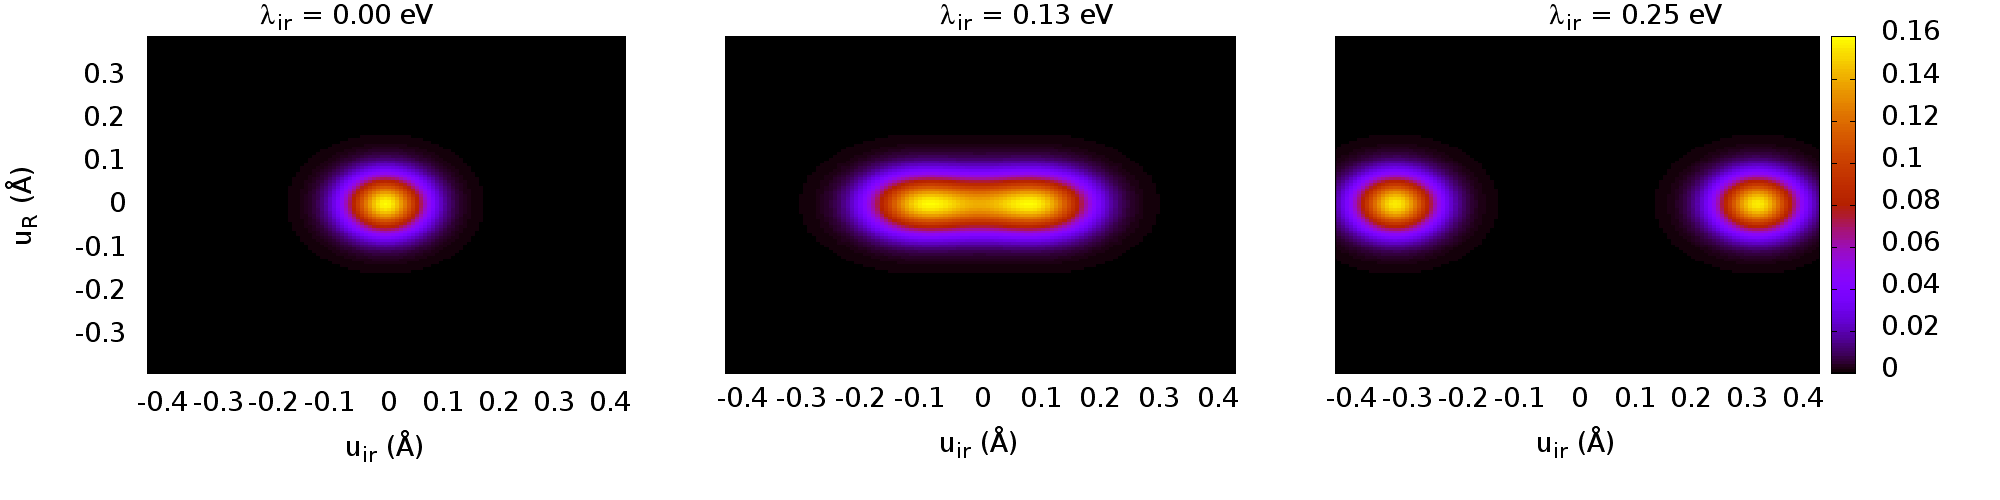
\includegraphics[width=0.8\textwidth]{images/ph-ground.png}
\caption{Ground state's projection into phonon coordinates.}
\label{fig:ph-ground}
\end{figure}

\section{Isotopic shift}

For the ground state we define the energy isotopic shift $\Delta_g$ in a similar way but with the energies measured relative to the uncoupled system (that is, the system with $\lambda_{ir}=\lambda_R=0$) (see \ref{isot-shift-def-grd}):

\begin{equation}
\Delta_g = \frac{\Delta E_g(^{16}O)- \Delta E_g(^{18}O)}{\Delta E_g(^{16}O)} \times 100 \end{equation}

where $\Delta E_g \equiv E_g - E_g(\lambda_{ir}=0, \lambda_R=0)$. To calculate this energies we need to take into account the *zero-point energy* in the phononic part $H_{ph}$ from (\ref{eq:full-hamiltonian}) writting it as \ref{phononic-part-complete}

The following figure plots this isotopic shift:

\begin{figure}[ht!]
\centering
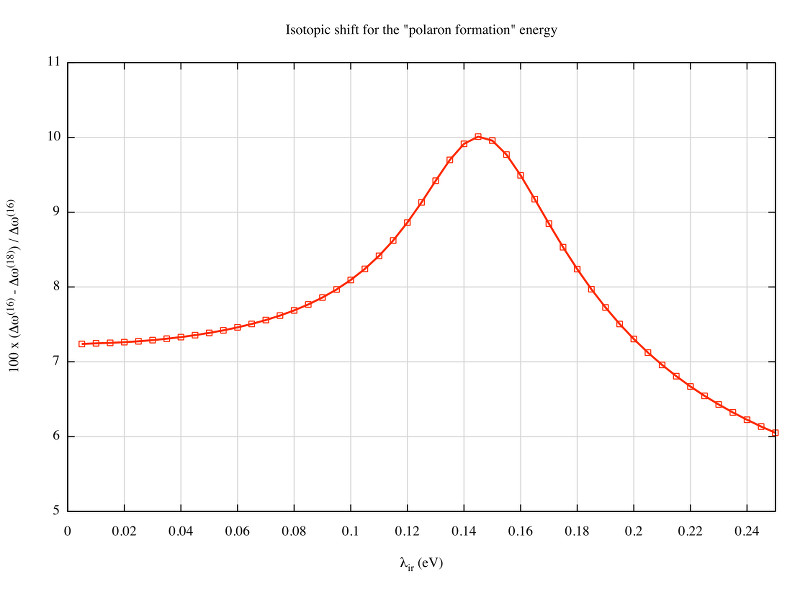
\includegraphics[width=0.8\textwidth]{images/isot_polaron_formation.jpg}
\caption{Isotopic shift of the polaron formation energy.}
\label{fig:isot_polaron_formation}
\end{figure}

Although $\Delta_g$ doesn't change sign, as the isotopic shift of the polaron tunneling state, it shows a maximum in the middle coupling regime reminiscent of the maximums, minimums or inflection points in the isotopic shifts for all the other excitations.
\chapter{States with more than one infrared phonons}

Section about the states with 2 and 3 infrared phonons and their particular behaviour.

\section{Energy renormalization}

At large $\lambda_{ir}$ we recover the harmonic behaviour. This is analog to have a spring with a displaced equilibrium position.

\section{Projection into phonon coordinates}

State with two infrared phonons:

\begin{figure}[ht!]
\centering
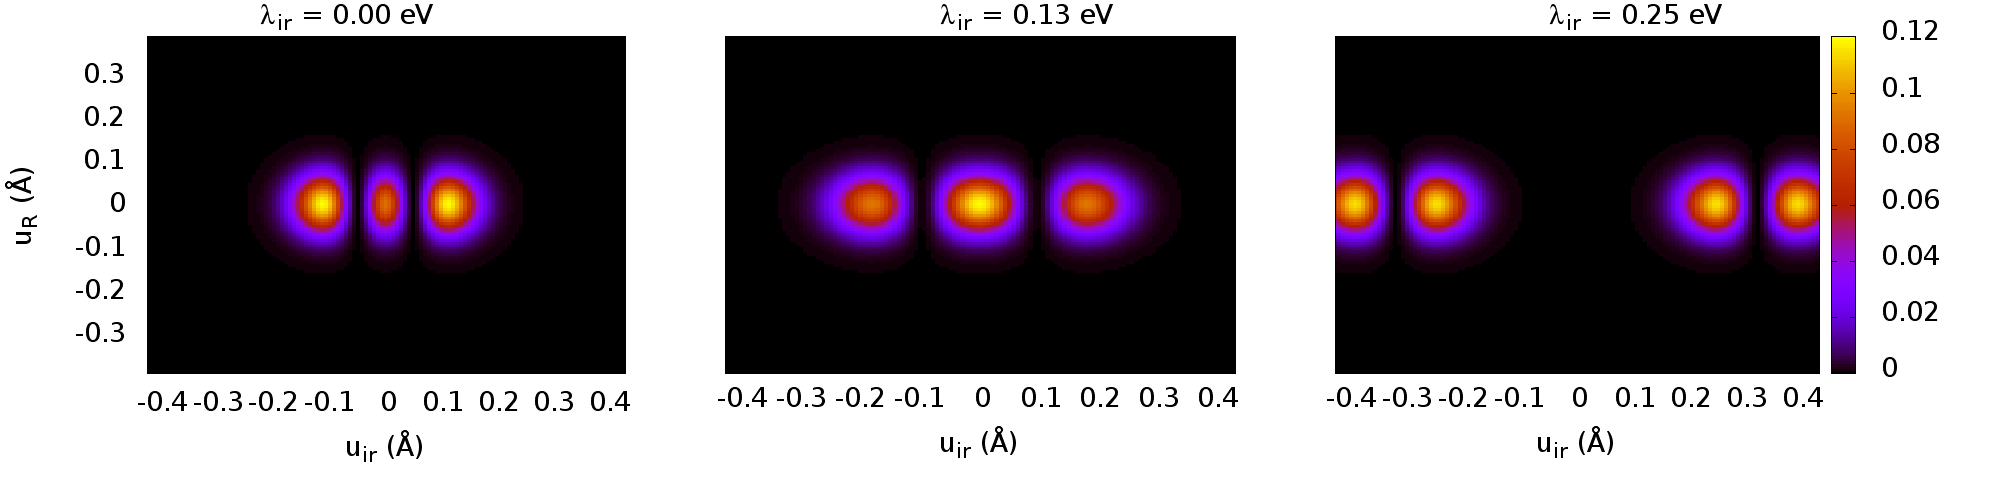
\includegraphics[width=0.8\textwidth]{images/ph-second_infrared.png}
\caption{Projection into phonon coordinates of the state with 2 infrared phonons.}
\label{fig:ph-second_infrared}
\end{figure}

State with three infrared phonons:

\begin{figure}[ht!]
\centering
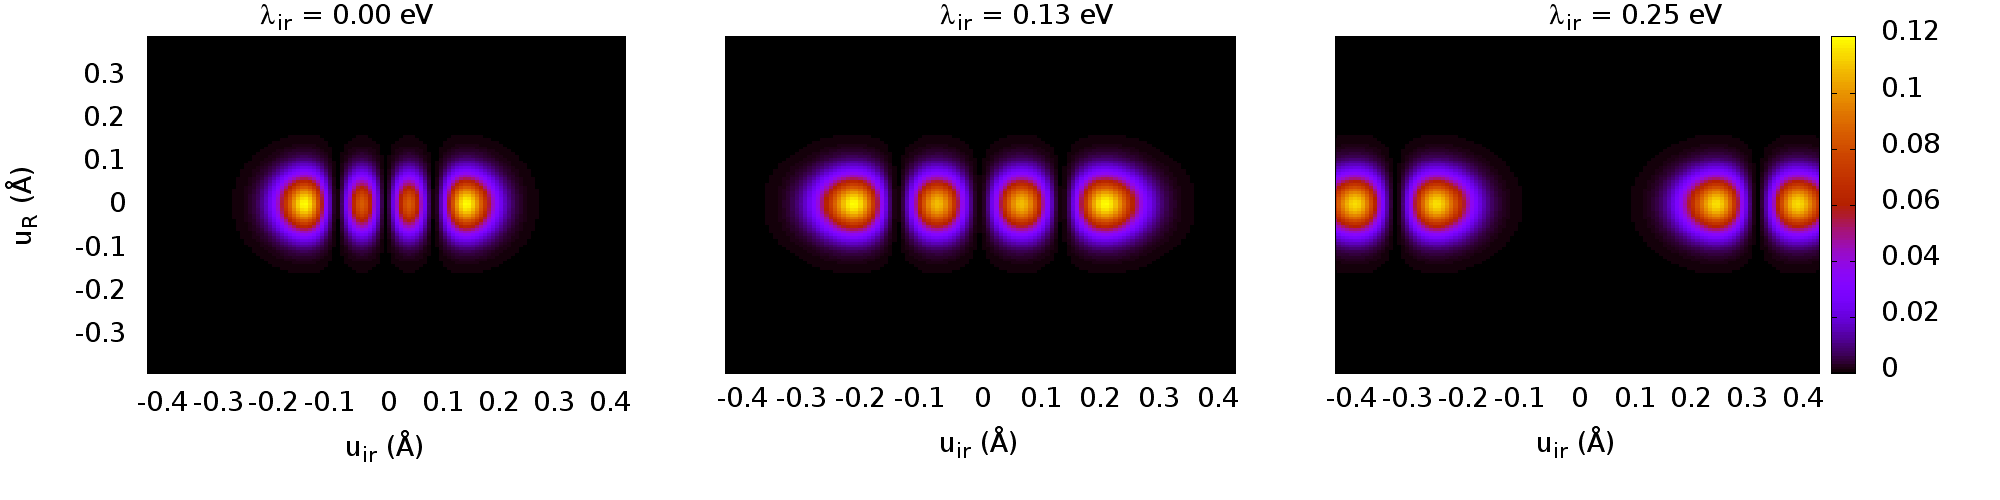
\includegraphics[width=0.8\textwidth]{images/ph-third_infrared.png}
\caption{Projection into phonon coordinates of the state with 3 infrared phonons.}
\label{fig:ph-third_infrared}
\end{figure}

\section{Isotopic shifts}

The isotopic shifts are different:

\begin{figure}[ht!]
\centering
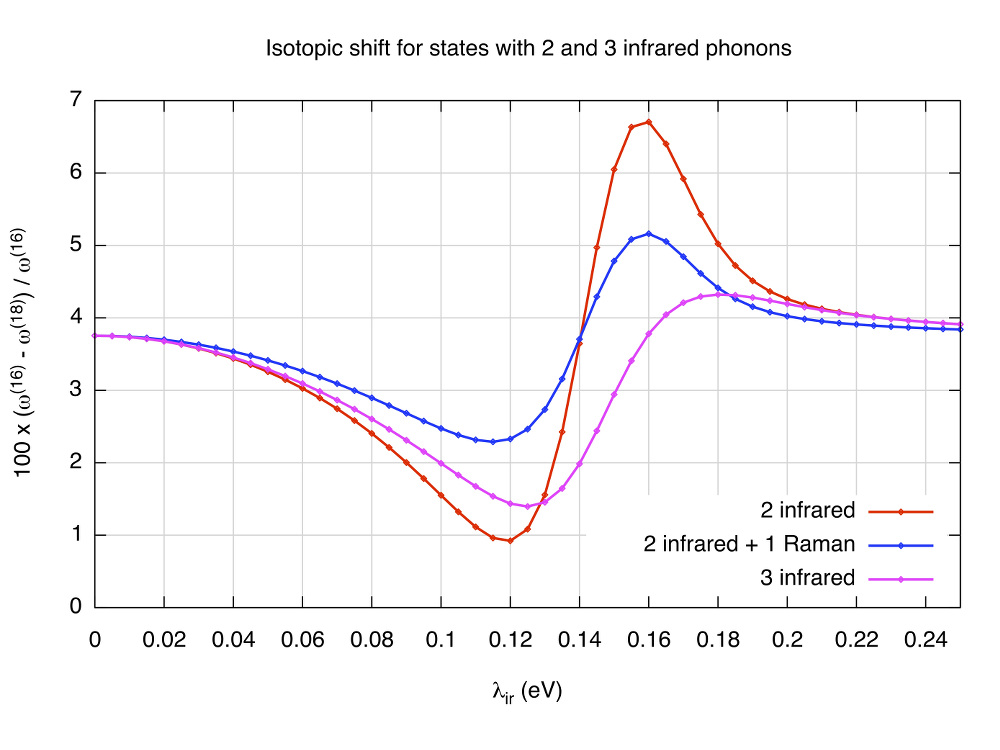
\includegraphics[width=0.8\textwidth]{images/isot-2_3ir.jpg}
\caption{Projection into phonon coordinates of the state with 3 infrared phonons.}
\label{fig:isot-2_3ir}
\end{figure}

\chapter{Electronic excitations}
\label{chap:electronic}

We call \textit{electronic} excitations those that, at $\lambda_{ir}=0$, arise from $H_{el}$ in (\ref{eq:full-hamiltonian}). This part of the hamiltonian

\begin{equation}\label{eq:Hel} H_{el} = \sum_n \epsilon_n \rho_n + \sum_{ \langle nm \rangle \sigma } t (c_{n \sigma }^\dagger c_{m \sigma } + H.c.) + U\sum_n \rho_{n\downarrow}\rho_{n\uparrow} \end{equation}

can be represented  as a 9x9 matrix:

\begin{equation}\label{eq:Hel-matrix} \left( \begin{array}{ccccccccc} 
U+2\epsilon &\;\;t\;\;&\;\;0\;\;&\;\;t\;\;&0&\;\;0\;\;&\;\;0\;\;&\;\;0\;\;&0 \\
t&0&t&0&t&0&0&0&0 \\
0&t&2\epsilon &0&0&t&0&0&0 \\
t&0&0&0&t&0&t&0&0 \\
0&t&0&t&U-2\epsilon &t&0&t&0 \\
0&0&t&0&t&0&0&0&t \\
0&0&0&t&0&0&2\epsilon &t&0 \\
0&0&0&0&t&0&t&0&t \\
0&0&0&0&0&t&0&t&U+2\epsilon  \end{array} \right)\end{equation}

and easily diagonalized to see that its first excited state has an energy of ~1376 cm$^{-1}$ above the  ground state.

\begin{figure}[ht]
  \centering
  % GNUPLOT: LaTeX picture with Postscript
\begingroup
  \makeatletter
  \providecommand\color[2][]{%
    \GenericError{(gnuplot) \space\space\space\@spaces}{%
      Package color not loaded in conjunction with
      terminal option `colourtext'%
    }{See the gnuplot documentation for explanation.%
    }{Either use 'blacktext' in gnuplot or load the package
      color.sty in LaTeX.}%
    \renewcommand\color[2][]{}%
  }%
  \providecommand\includegraphics[2][]{%
    \GenericError{(gnuplot) \space\space\space\@spaces}{%
      Package graphicx or graphics not loaded%
    }{See the gnuplot documentation for explanation.%
    }{The gnuplot epslatex terminal needs graphicx.sty or graphics.sty.}%
    \renewcommand\includegraphics[2][]{}%
  }%
  \providecommand\rotatebox[2]{#2}%
  \@ifundefined{ifGPcolor}{%
    \newif\ifGPcolor
    \GPcolortrue
  }{}%
  \@ifundefined{ifGPblacktext}{%
    \newif\ifGPblacktext
    \GPblacktextfalse
  }{}%
  % define a \g@addto@macro without @ in the name:
  \let\gplgaddtomacro\g@addto@macro
  % define empty templates for all commands taking text:
  \gdef\gplbacktext{}%
  \gdef\gplfronttext{}%
  \makeatother
  \ifGPblacktext
    % no textcolor at all
    \def\colorrgb#1{}%
    \def\colorgray#1{}%
  \else
    % gray or color?
    \ifGPcolor
      \def\colorrgb#1{\color[rgb]{#1}}%
      \def\colorgray#1{\color[gray]{#1}}%
      \expandafter\def\csname LTw\endcsname{\color{white}}%
      \expandafter\def\csname LTb\endcsname{\color{black}}%
      \expandafter\def\csname LTa\endcsname{\color{black}}%
      \expandafter\def\csname LT0\endcsname{\color[rgb]{1,0,0}}%
      \expandafter\def\csname LT1\endcsname{\color[rgb]{0,1,0}}%
      \expandafter\def\csname LT2\endcsname{\color[rgb]{0,0,1}}%
      \expandafter\def\csname LT3\endcsname{\color[rgb]{1,0,1}}%
      \expandafter\def\csname LT4\endcsname{\color[rgb]{0,1,1}}%
      \expandafter\def\csname LT5\endcsname{\color[rgb]{1,1,0}}%
      \expandafter\def\csname LT6\endcsname{\color[rgb]{0,0,0}}%
      \expandafter\def\csname LT7\endcsname{\color[rgb]{1,0.3,0}}%
      \expandafter\def\csname LT8\endcsname{\color[rgb]{0.5,0.5,0.5}}%
    \else
      % gray
      \def\colorrgb#1{\color{black}}%
      \def\colorgray#1{\color[gray]{#1}}%
      \expandafter\def\csname LTw\endcsname{\color{white}}%
      \expandafter\def\csname LTb\endcsname{\color{black}}%
      \expandafter\def\csname LTa\endcsname{\color{black}}%
      \expandafter\def\csname LT0\endcsname{\color{black}}%
      \expandafter\def\csname LT1\endcsname{\color{black}}%
      \expandafter\def\csname LT2\endcsname{\color{black}}%
      \expandafter\def\csname LT3\endcsname{\color{black}}%
      \expandafter\def\csname LT4\endcsname{\color{black}}%
      \expandafter\def\csname LT5\endcsname{\color{black}}%
      \expandafter\def\csname LT6\endcsname{\color{black}}%
      \expandafter\def\csname LT7\endcsname{\color{black}}%
      \expandafter\def\csname LT8\endcsname{\color{black}}%
    \fi
  \fi
  \setlength{\unitlength}{0.0500bp}%
  \begin{picture}(6802.00,4534.00)%
    \gplgaddtomacro\gplbacktext{%
      \colorrgb{0.31,0.31,0.31}%
      \put(1210,751){\makebox(0,0)[r]{\strut{}\scriptsize 1000}}%
      \colorrgb{0.31,0.31,0.31}%
      \put(1210,1631){\makebox(0,0)[r]{\strut{}\scriptsize 1250}}%
      \colorrgb{0.31,0.31,0.31}%
      \put(1210,2510){\makebox(0,0)[r]{\strut{}\scriptsize 1500}}%
      \colorrgb{0.31,0.31,0.31}%
      \put(1210,3390){\makebox(0,0)[r]{\strut{}\scriptsize 1750}}%
      \colorrgb{0.31,0.31,0.31}%
      \put(1210,4269){\makebox(0,0)[r]{\strut{}\scriptsize 2000}}%
      \colorrgb{0.31,0.31,0.31}%
      \put(1389,484){\makebox(0,0){\strut{}\scriptsize 0}}%
      \colorrgb{0.31,0.31,0.31}%
      \put(1790,484){\makebox(0,0){\strut{}\scriptsize 0.02}}%
      \colorrgb{0.31,0.31,0.31}%
      \put(2192,484){\makebox(0,0){\strut{}\scriptsize 0.04}}%
      \colorrgb{0.31,0.31,0.31}%
      \put(2593,484){\makebox(0,0){\strut{}\scriptsize 0.06}}%
      \colorrgb{0.31,0.31,0.31}%
      \put(2994,484){\makebox(0,0){\strut{}\scriptsize 0.08}}%
      \colorrgb{0.31,0.31,0.31}%
      \put(3395,484){\makebox(0,0){\strut{}\scriptsize 0.1}}%
      \colorrgb{0.31,0.31,0.31}%
      \put(3797,484){\makebox(0,0){\strut{}\scriptsize 0.12}}%
      \colorrgb{0.31,0.31,0.31}%
      \put(4198,484){\makebox(0,0){\strut{}\scriptsize 0.14}}%
      \colorrgb{0.31,0.31,0.31}%
      \put(4599,484){\makebox(0,0){\strut{}\scriptsize 0.16}}%
      \colorrgb{0.31,0.31,0.31}%
      \put(5001,484){\makebox(0,0){\strut{}\scriptsize 0.18}}%
      \colorrgb{0.31,0.31,0.31}%
      \put(5402,484){\makebox(0,0){\strut{}\scriptsize 0.2}}%
      \colorrgb{0.31,0.31,0.31}%
      \put(5803,484){\makebox(0,0){\strut{}\scriptsize 0.22}}%
      \colorrgb{0.31,0.31,0.31}%
      \put(6204,484){\makebox(0,0){\strut{}\scriptsize 0.24}}%
      \csname LTb\endcsname%
      \put(176,2510){\rotatebox{-270}{\makebox(0,0){\strut{}$\omega_i$ (cm$^{-1}$)}}}%
      \put(3897,154){\makebox(0,0){\strut{}$\lambda_{ir}$ (eV)}}%
      \put(3997,3988){\makebox(0,0)[l]{\strut{}\scriptsize$\lambda_{ir}=0.1263$}}%
    }%
    \gplgaddtomacro\gplfronttext{%
    }%
    \gplbacktext
    \put(0,0){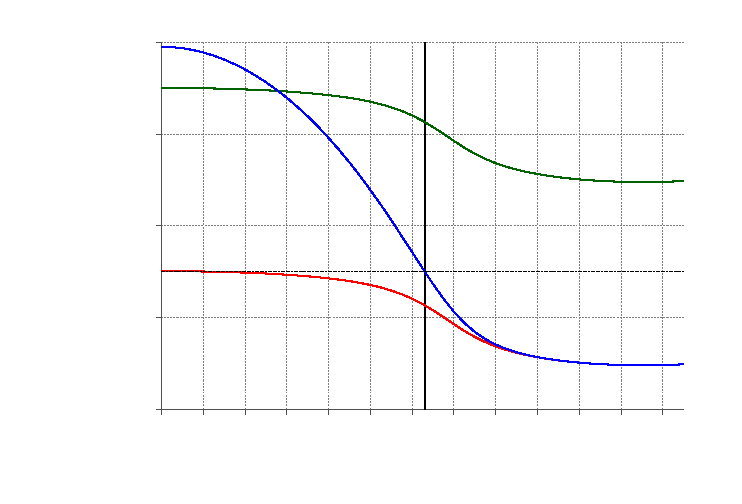
\includegraphics{images/electrSpectra}}%
    \gplfronttext
  \end{picture}%
\endgroup

  \caption[Energy of the electronic excitations as function of $\lambda_{ir}$.]
  {Energy of the electronic excitations as function of $\lambda_{ir}$. 
    The red line corresponds to an electronic excitation with zero phonons, the blue line with one infrared phonon and the green line with one Raman phonon.
    The vertical line is placed at the relevant value $\lambda_{ir}=0.1263$ eV.}
  \label{fig:electrSpectra}
\end{figure}

\section{Projection into definite electronic occupation states}

Since we are using basis states with definite electron occupancy, from the eigenvectors of the (\ref{eq:Hel-matrix}) matrix we can directly see the projections into definite electronic occupation states. The following table summarizes those values omitting equivalent basis states:

\noindent\begin{tabular}{| c | c | c | c | c | c | c | c | c | c |}
\hline
Energy (cm$^{-1}$) & 0.0 & 1376.42 & 3825.49 & 4325.12 & 14897.84 & 15329.82 & 53933.30 & 69272.75 & 69309.3 \\
\hline
$\uparrow \downarrow \ - \ -$ & 0.00276 & 0.00000 & 0.00382 & 0.00000 & 0.00090 & 0.00000 & 0.00179 & 0.49618 & 0.49455 \\
$\uparrow\  \downarrow \ -$ & 0.20130 & 0.19717 & 0.24809 & 0.25000 & 0.04045 & 0.05283 & 0.00606 & 0.00191 & 0.00219 \\
$\uparrow \ - \ \downarrow$ & 0.08522 & 0.10566 & 0.00000 & 0.00000 & 0.41451 & 0.39434 & 0.00023 & 0.00000 & 0.00000 \\
$ - \ \uparrow \downarrow \ -$ & 0.01884 & 0.00000 & 0.00000 & 0.00000 & 0.00736 & 0.00000 & 0.97174 & 0.00000 & 0.00205 \\
\hline
\end{tabular}

We noticed\cite{GarciaSaraviaOrtizdeMontellano2013} that, for the first \textit{electronic} excitation, the projection into states with an electron in each oxygen decreases with an increasing $\lambda_{ir}$ suggesting partial charge localization.

\section{Projection into phonon coordinates}

\begin{figure}[ht]
  \centering
  % GNUPLOT: LaTeX picture with Postscript
\begingroup
  \makeatletter
  \providecommand\color[2][]{%
    \GenericError{(gnuplot) \space\space\space\@spaces}{%
      Package color not loaded in conjunction with
      terminal option `colourtext'%
    }{See the gnuplot documentation for explanation.%
    }{Either use 'blacktext' in gnuplot or load the package
      color.sty in LaTeX.}%
    \renewcommand\color[2][]{}%
  }%
  \providecommand\includegraphics[2][]{%
    \GenericError{(gnuplot) \space\space\space\@spaces}{%
      Package graphicx or graphics not loaded%
    }{See the gnuplot documentation for explanation.%
    }{The gnuplot epslatex terminal needs graphicx.sty or graphics.sty.}%
    \renewcommand\includegraphics[2][]{}%
  }%
  \providecommand\rotatebox[2]{#2}%
  \@ifundefined{ifGPcolor}{%
    \newif\ifGPcolor
    \GPcolortrue
  }{}%
  \@ifundefined{ifGPblacktext}{%
    \newif\ifGPblacktext
    \GPblacktextfalse
  }{}%
  % define a \g@addto@macro without @ in the name:
  \let\gplgaddtomacro\g@addto@macro
  % define empty templates for all commands taking text:
  \gdef\gplbacktext{}%
  \gdef\gplfronttext{}%
  \makeatother
  \ifGPblacktext
    % no textcolor at all
    \def\colorrgb#1{}%
    \def\colorgray#1{}%
  \else
    % gray or color?
    \ifGPcolor
      \def\colorrgb#1{\color[rgb]{#1}}%
      \def\colorgray#1{\color[gray]{#1}}%
      \expandafter\def\csname LTw\endcsname{\color{white}}%
      \expandafter\def\csname LTb\endcsname{\color{black}}%
      \expandafter\def\csname LTa\endcsname{\color{black}}%
      \expandafter\def\csname LT0\endcsname{\color[rgb]{1,0,0}}%
      \expandafter\def\csname LT1\endcsname{\color[rgb]{0,1,0}}%
      \expandafter\def\csname LT2\endcsname{\color[rgb]{0,0,1}}%
      \expandafter\def\csname LT3\endcsname{\color[rgb]{1,0,1}}%
      \expandafter\def\csname LT4\endcsname{\color[rgb]{0,1,1}}%
      \expandafter\def\csname LT5\endcsname{\color[rgb]{1,1,0}}%
      \expandafter\def\csname LT6\endcsname{\color[rgb]{0,0,0}}%
      \expandafter\def\csname LT7\endcsname{\color[rgb]{1,0.3,0}}%
      \expandafter\def\csname LT8\endcsname{\color[rgb]{0.5,0.5,0.5}}%
    \else
      % gray
      \def\colorrgb#1{\color{black}}%
      \def\colorgray#1{\color[gray]{#1}}%
      \expandafter\def\csname LTw\endcsname{\color{white}}%
      \expandafter\def\csname LTb\endcsname{\color{black}}%
      \expandafter\def\csname LTa\endcsname{\color{black}}%
      \expandafter\def\csname LT0\endcsname{\color{black}}%
      \expandafter\def\csname LT1\endcsname{\color{black}}%
      \expandafter\def\csname LT2\endcsname{\color{black}}%
      \expandafter\def\csname LT3\endcsname{\color{black}}%
      \expandafter\def\csname LT4\endcsname{\color{black}}%
      \expandafter\def\csname LT5\endcsname{\color{black}}%
      \expandafter\def\csname LT6\endcsname{\color{black}}%
      \expandafter\def\csname LT7\endcsname{\color{black}}%
      \expandafter\def\csname LT8\endcsname{\color{black}}%
    \fi
  \fi
  \setlength{\unitlength}{0.0500bp}%
  \begin{picture}(7936.00,2834.00)%
    \gplgaddtomacro\gplbacktext{%
      \csname LTb\endcsname%
      \put(-63,879){\makebox(0,0)[r]{\strut{}\scriptsize -0.3}}%
      \put(-63,1124){\makebox(0,0)[r]{\strut{}\scriptsize -0.2}}%
      \put(-63,1369){\makebox(0,0)[r]{\strut{}\scriptsize -0.1}}%
      \put(-63,1615){\makebox(0,0)[r]{\strut{}\scriptsize 0}}%
      \put(-63,1860){\makebox(0,0)[r]{\strut{}\scriptsize 0.1}}%
      \put(-63,2105){\makebox(0,0)[r]{\strut{}\scriptsize 0.2}}%
      \put(-63,2350){\makebox(0,0)[r]{\strut{}\scriptsize 0.3}}%
      \put(218,377){\makebox(0,0){\strut{}\scriptsize -0.4}}%
      \put(764,377){\makebox(0,0){\strut{}\scriptsize -0.2}}%
      \put(1309,377){\makebox(0,0){\strut{}\scriptsize 0}}%
      \put(1854,377){\makebox(0,0){\strut{}\scriptsize 0.2}}%
      \put(2400,377){\makebox(0,0){\strut{}\scriptsize 0.4}}%
      \put(-569,1614){\rotatebox{-270}{\makebox(0,0){\strut{}$u_{R}$ (\AA)}}}%
      \put(1309,91){\makebox(0,0){\strut{}}}%
      \put(794,2720){\makebox(0,0)[l]{\strut{}\scriptsize{$\lambda_{ir} = 0.00$ eV}}}%
    }%
    \gplgaddtomacro\gplfronttext{%
    }%
    \gplgaddtomacro\gplbacktext{%
      \csname LTb\endcsname%
      \put(2836,377){\makebox(0,0){\strut{}\scriptsize -0.4}}%
      \put(3382,377){\makebox(0,0){\strut{}\scriptsize -0.2}}%
      \put(3928,377){\makebox(0,0){\strut{}\scriptsize 0}}%
      \put(4473,377){\makebox(0,0){\strut{}\scriptsize 0.2}}%
      \put(5019,377){\makebox(0,0){\strut{}\scriptsize 0.4}}%
      \put(3278,1614){\rotatebox{-270}{\makebox(0,0){\strut{}}}}%
      \put(3927,47){\makebox(0,0){\strut{}$u_{ir}$ (\AA)}}%
      \put(3412,2720){\makebox(0,0)[l]{\strut{}\scriptsize{$\lambda_{ir} = 0.1263$ eV}}}%
    }%
    \gplgaddtomacro\gplfronttext{%
    }%
    \gplgaddtomacro\gplbacktext{%
      \csname LTb\endcsname%
      \put(5455,377){\makebox(0,0){\strut{}\scriptsize -0.4}}%
      \put(6001,377){\makebox(0,0){\strut{}\scriptsize -0.2}}%
      \put(6546,377){\makebox(0,0){\strut{}\scriptsize 0}}%
      \put(7091,377){\makebox(0,0){\strut{}\scriptsize 0.2}}%
      \put(7637,377){\makebox(0,0){\strut{}\scriptsize 0.4}}%
      \put(5897,1614){\rotatebox{-270}{\makebox(0,0){\strut{}}}}%
      \put(6546,91){\makebox(0,0){\strut{}}}%
      \put(6031,2720){\makebox(0,0)[l]{\strut{}\scriptsize{$\lambda_{ir} = 0.25$ eV}}}%
    }%
    \gplgaddtomacro\gplfronttext{%
    }%
    \gplbacktext
    \put(0,0){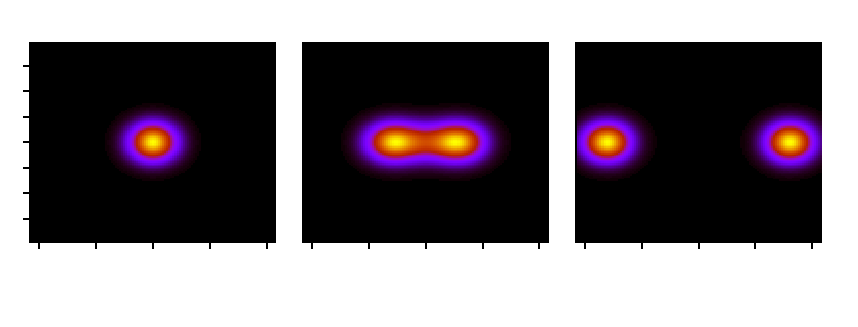
\includegraphics{images/phononProjElectr}}%
    \gplfronttext
  \end{picture}%
\endgroup

  \caption{Electronic state projected into phonon coordinates for three representative electron-lattice coupling ($\lambda_{ir}$) values.}
  \label{fig:phononProjElectr}
\end{figure}

\section{Isotopic shift}

\begin{figure}[ht]
  \centering
  % GNUPLOT: LaTeX picture with Postscript
\begingroup
  \makeatletter
  \providecommand\color[2][]{%
    \GenericError{(gnuplot) \space\space\space\@spaces}{%
      Package color not loaded in conjunction with
      terminal option `colourtext'%
    }{See the gnuplot documentation for explanation.%
    }{Either use 'blacktext' in gnuplot or load the package
      color.sty in LaTeX.}%
    \renewcommand\color[2][]{}%
  }%
  \providecommand\includegraphics[2][]{%
    \GenericError{(gnuplot) \space\space\space\@spaces}{%
      Package graphicx or graphics not loaded%
    }{See the gnuplot documentation for explanation.%
    }{The gnuplot epslatex terminal needs graphicx.sty or graphics.sty.}%
    \renewcommand\includegraphics[2][]{}%
  }%
  \providecommand\rotatebox[2]{#2}%
  \@ifundefined{ifGPcolor}{%
    \newif\ifGPcolor
    \GPcolortrue
  }{}%
  \@ifundefined{ifGPblacktext}{%
    \newif\ifGPblacktext
    \GPblacktextfalse
  }{}%
  % define a \g@addto@macro without @ in the name:
  \let\gplgaddtomacro\g@addto@macro
  % define empty templates for all commands taking text:
  \gdef\gplbacktext{}%
  \gdef\gplfronttext{}%
  \makeatother
  \ifGPblacktext
    % no textcolor at all
    \def\colorrgb#1{}%
    \def\colorgray#1{}%
  \else
    % gray or color?
    \ifGPcolor
      \def\colorrgb#1{\color[rgb]{#1}}%
      \def\colorgray#1{\color[gray]{#1}}%
      \expandafter\def\csname LTw\endcsname{\color{white}}%
      \expandafter\def\csname LTb\endcsname{\color{black}}%
      \expandafter\def\csname LTa\endcsname{\color{black}}%
      \expandafter\def\csname LT0\endcsname{\color[rgb]{1,0,0}}%
      \expandafter\def\csname LT1\endcsname{\color[rgb]{0,1,0}}%
      \expandafter\def\csname LT2\endcsname{\color[rgb]{0,0,1}}%
      \expandafter\def\csname LT3\endcsname{\color[rgb]{1,0,1}}%
      \expandafter\def\csname LT4\endcsname{\color[rgb]{0,1,1}}%
      \expandafter\def\csname LT5\endcsname{\color[rgb]{1,1,0}}%
      \expandafter\def\csname LT6\endcsname{\color[rgb]{0,0,0}}%
      \expandafter\def\csname LT7\endcsname{\color[rgb]{1,0.3,0}}%
      \expandafter\def\csname LT8\endcsname{\color[rgb]{0.5,0.5,0.5}}%
    \else
      % gray
      \def\colorrgb#1{\color{black}}%
      \def\colorgray#1{\color[gray]{#1}}%
      \expandafter\def\csname LTw\endcsname{\color{white}}%
      \expandafter\def\csname LTb\endcsname{\color{black}}%
      \expandafter\def\csname LTa\endcsname{\color{black}}%
      \expandafter\def\csname LT0\endcsname{\color{black}}%
      \expandafter\def\csname LT1\endcsname{\color{black}}%
      \expandafter\def\csname LT2\endcsname{\color{black}}%
      \expandafter\def\csname LT3\endcsname{\color{black}}%
      \expandafter\def\csname LT4\endcsname{\color{black}}%
      \expandafter\def\csname LT5\endcsname{\color{black}}%
      \expandafter\def\csname LT6\endcsname{\color{black}}%
      \expandafter\def\csname LT7\endcsname{\color{black}}%
      \expandafter\def\csname LT8\endcsname{\color{black}}%
    \fi
  \fi
  \setlength{\unitlength}{0.0500bp}%
  \begin{picture}(6802.00,4534.00)%
    \gplgaddtomacro\gplbacktext{%
      \colorrgb{0.31,0.31,0.31}%
      \put(1210,751){\makebox(0,0)[r]{\strut{}\scriptsize -2}}%
      \colorrgb{0.31,0.31,0.31}%
      \put(1210,1191){\makebox(0,0)[r]{\strut{}\scriptsize -1.5}}%
      \colorrgb{0.31,0.31,0.31}%
      \put(1210,1631){\makebox(0,0)[r]{\strut{}\scriptsize -1}}%
      \colorrgb{0.31,0.31,0.31}%
      \put(1210,2070){\makebox(0,0)[r]{\strut{}\scriptsize -0.5}}%
      \colorrgb{0.31,0.31,0.31}%
      \put(1210,2510){\makebox(0,0)[r]{\strut{}\scriptsize 0}}%
      \colorrgb{0.31,0.31,0.31}%
      \put(1210,2950){\makebox(0,0)[r]{\strut{}\scriptsize 0.5}}%
      \colorrgb{0.31,0.31,0.31}%
      \put(1210,3390){\makebox(0,0)[r]{\strut{}\scriptsize 1}}%
      \colorrgb{0.31,0.31,0.31}%
      \put(1210,3829){\makebox(0,0)[r]{\strut{}\scriptsize 1.5}}%
      \colorrgb{0.31,0.31,0.31}%
      \put(1210,4269){\makebox(0,0)[r]{\strut{}\scriptsize 2}}%
      \colorrgb{0.31,0.31,0.31}%
      \put(1389,484){\makebox(0,0){\strut{}\scriptsize 0}}%
      \colorrgb{0.31,0.31,0.31}%
      \put(1790,484){\makebox(0,0){\strut{}\scriptsize 0.02}}%
      \colorrgb{0.31,0.31,0.31}%
      \put(2192,484){\makebox(0,0){\strut{}\scriptsize 0.04}}%
      \colorrgb{0.31,0.31,0.31}%
      \put(2593,484){\makebox(0,0){\strut{}\scriptsize 0.06}}%
      \colorrgb{0.31,0.31,0.31}%
      \put(2994,484){\makebox(0,0){\strut{}\scriptsize 0.08}}%
      \colorrgb{0.31,0.31,0.31}%
      \put(3395,484){\makebox(0,0){\strut{}\scriptsize 0.1}}%
      \colorrgb{0.31,0.31,0.31}%
      \put(3797,484){\makebox(0,0){\strut{}\scriptsize 0.12}}%
      \colorrgb{0.31,0.31,0.31}%
      \put(4198,484){\makebox(0,0){\strut{}\scriptsize 0.14}}%
      \colorrgb{0.31,0.31,0.31}%
      \put(4599,484){\makebox(0,0){\strut{}\scriptsize 0.16}}%
      \colorrgb{0.31,0.31,0.31}%
      \put(5001,484){\makebox(0,0){\strut{}\scriptsize 0.18}}%
      \colorrgb{0.31,0.31,0.31}%
      \put(5402,484){\makebox(0,0){\strut{}\scriptsize 0.2}}%
      \colorrgb{0.31,0.31,0.31}%
      \put(5803,484){\makebox(0,0){\strut{}\scriptsize 0.22}}%
      \colorrgb{0.31,0.31,0.31}%
      \put(6204,484){\makebox(0,0){\strut{}\scriptsize 0.24}}%
      \csname LTb\endcsname%
      \put(176,2510){\rotatebox{-270}{\makebox(0,0){\strut{}$\omega_i$ (cm$^{-1}$)}}}%
      \put(3897,154){\makebox(0,0){\strut{}$\lambda_{ir}$ (eV)}}%
      \put(3997,3988){\makebox(0,0)[l]{\strut{}\scriptsize$\lambda_{ir}=0.1263$}}%
    }%
    \gplgaddtomacro\gplfronttext{%
    }%
    \gplbacktext
    \put(0,0){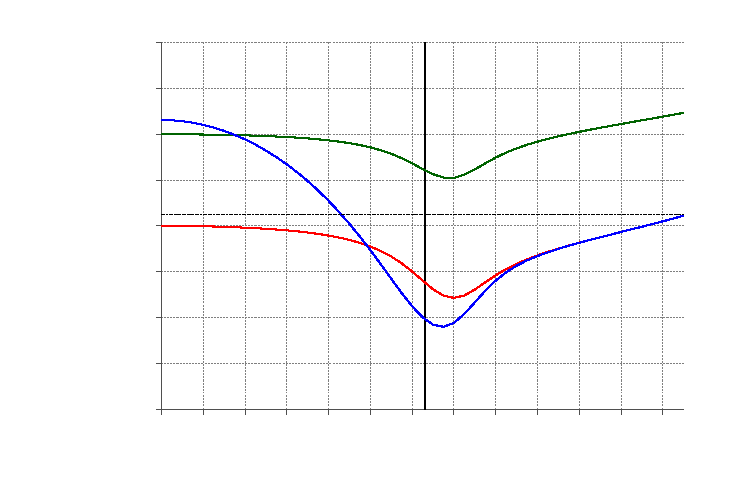
\includegraphics{images/electrIsot}}%
    \gplfronttext
  \end{picture}%
\endgroup

  \caption[Isotopic shift of the electronic excitations as a function of $\lambda_{ir}$.]
  {Isotopic shifts of the electronic excitations as a function of $\lambda_{ir}$. 
    The red line corresponds to an electronic excitation with zero phonons, the blue line with one infrared phonon and the green line with one Raman phonon.
    The vertical line is placed at the relevant value $\lambda_{ir}=0.1263$ eV.}
  \label{fig:electrIsot}
\end{figure}


\chapter{Discussion and conclusions}
\label{chap:conclusions}

We have reviewed the evidence for the appearance of a dynamically inhomogeneous ground state in the pseudogap region. In this state there are bipolaronic objects which form at a characteristic temperature T*. The manifestations of these objects in the lattice appear as dynamical local lattice distortions in regions in which the charge and lattice motion become correlated. The excitations of these bipolaronic objects exhibit different isotopic shifts depending on the nature of the excitation ranging from large negative to quasi-harmonic shifts. These peculiar shifts are consistent with experimental observations and might explain discrepancies in values determined by different techniques, as they probe different excitations depending on the time and spatial resolution of the specific technique. The role in the pairing of free fermions of these bipolaronic excitations, and enhancement of T$_c$ is not yet known. In this spirit, some models have considered the interaction between fermionic *pairs* and bipolaronic bosonic objects [Mihailovic 01] [Ba-Yam 90] [Bussmann-Holder 05] [Bianconi 00] explaining several properties of the normal state in this pseudogap region.  Here, we have presented a natural extension of the model treated,  coupling the bipolaronic subsystem to an independent a free fermion subsystem, and discussed a signature of pairing of fermions. Additionally, the role played by the antiferromagnetic background present at zero doping and its interaction with both the fermionic carriers and polaronic objects has to be addressed.

\section{Validity of the Born-Oppenheimer approximation}

It is interesting to note that, although the isotopic shifts of the ground state and lowest excitations can be either positive or negative, they all exhibit the strongest variations in the intermediate coupling regime suggesting a characteristic dynamical scale for the polaronic features. Other transition metals oxides as manganites and nickelates exhibit similar local lattice distortions.  However, the size of the distortion is far larger in manganites (~0.2 \AA) [Tyson96]  and smaller in nickelates (~0.05 \AA) [Acosta08] resulting also in different time scales. It is enticing to relate the particular dynamical time scale of the local lattice distortions with the presence of high-temperature superconductivity in cuprates but not in other transition metal oxides. We stress that in this intermediate coupling region other treatments like adiabatic or anti-adiabatic approximations are unable to describe the specific features of the polaronic system found with the exact treatment on a small cluster.

\section{Multicomponent superconductivity}

Finally, we would like to discuss the possible relevance of the bipolaronic behavior, derived from the simple Peierls-Hubbard Hamiltonian model to high temperature superconductivity. The observation of a Fermi surface in photoemission experiments [Ding 96] [Hussey 03] implies that in addition to the bipolaronic objects (of bosonic character) there are also quasi-free fermions. As a function of doping the ratio of these two kinds of objects varies, yielding different characterizations of the ground state starting as an antiferromagnetic Mott insulator at zero doping, an inhomogeneous pseudogap phase where at least two different type of carriers coexist and ending in a Fermi-liquid metal in the overdoped region of the phase diagram. The fact that the highest T$_c$  is realized in this pseudogap region highlights the importance of the bipolaron bosonic objects. However, their role in the pairing of free fermions and enhancement of T$_c$ is not yet known. In order to understand this role, a natural extension of the model treated here is to couple the Halmiltonian  (\ref{full-hamiltonian}) to an independent a free fermion system $H_A$ and find the corresponding excitations allowing exchange of the fermions involved in the bipolaronic objects with those in the free fermion part. In the spirit of the exact treatment of the bipolaronic subsystem,  the simplest interaction between mobile fermions and charges forming part of a bipolaron is a linear hopping term. Such term would allow transfer of a single fermion from the mobile fermion and the bipolaron subsystems.  In principle in an exact treatment the possibility of pair hopping would be implicitly included. That is not the case in a perturbative treatment, in which the single particle exchange (hoping) can be folded into the pair exchange. See reference [Ba-Yam 90].

\begin{equation}
\label{eq:multicomponent}
H_A = 
E_A \sum_{\sigma, k=1,2} m_{\sigma, k} + 
t_A \sum_{\sigma} (a_{\sigma, 1}^\dagger a_{\sigma, 2} + a_{\sigma,2}^\dagger a_{\sigma, 1}) + 
\lambda_A \sum_{i,k,\sigma} \left( c_{i,\sigma}^\dagger a_{k,\sigma} + a_{k,\sigma}^\dagger c_{i,\sigma} \right) \end{equation}
%
with $i=1,2,3$ labeling the sites in the O-Cu-O cluster and $k=1,2$ the two sites for the free fermions. Where $m_{\sigma, k} = a_{\sigma, k}^\dagger a_{\sigma, k}$.
As the simplest model of the free fermion subsystem, we have this two site system with two non interacting fermions. This approach still allows us to use an exact treatment of the model, albeit missing the possible extended nature of the free fermion states. If a perturbative approach was used instead it could be possible to replace the free fermion subsystem by a full band in $k$-space. In addition an onsite Coulomb repulsion term could be added to the free electron subsystem and still perform an exact diagonalization.  In this case the used basis set is two orders of magnitude larger than for the original Peirles-Hubbard Hamiltonian (\ref{full-hamiltonian}). In this model an increased projection of a given excitation on a double occupancy basis state of the free fermion part  would be a signature of pairing. We are still searching for such signature in this model.


\appendix
%\include{filename}

% Bibliography
\cleardoublepage
\bibliography{biblio}
\addcontentsline{toc}{chapter}{\bibname}
\bibliographystyle{unsrt}

% Subject index
\addcontentsline{toc}{chapter}{Subject index}
\printindex

\end{document}
